% =====================================================================
%  YOPO 技术汇报 —— 前向推理 / 引导训练
%  编译：xelatex -> xelatex（需要 ctex/beamer；第二次编译页码才正确）
%  依据：YOPO/papernote.md（2026-10-08）与原文 PDF
% =====================================================================
% !TEX program = xelatex
\documentclass[aspectratio=169,11pt]{beamer}

% ---------- 中文与数学 ----------
\usepackage[UTF8]{ctex}
\usepackage{amsmath,amssymb}
\usepackage{booktabs}
\usepackage{array}
\usepackage{multirow}
\usepackage{graphicx}
\usepackage{tikz}
\usetikzlibrary{positioning,arrows.meta,calc,decorations.pathreplacing}

% ---------- 配色 ----------
\definecolor{yopoblue}{HTML}{1F4E79}
\definecolor{yopomid}{HTML}{2E75B6}
\definecolor{yopoorange}{HTML}{D2691E}
\definecolor{yopogreen}{HTML}{2E8B57}
\definecolor{yopogray}{HTML}{5A5A5A}
\definecolor{yopopale}{HTML}{EEF3F8}
\definecolor{yopowarm}{HTML}{FDF3E7}

% ---------- 主题 ----------
\usetheme{default}
\useinnertheme{rectangles}
\setbeamertemplate{navigation symbols}{}
\setbeamercolor{structure}{fg=yopoblue}
\setbeamercolor{frametitle}{bg=yopoblue,fg=white}
\setbeamercolor{title}{fg=yopoblue}
\setbeamercolor{subtitle}{fg=yopogray}
\setbeamercolor{block title}{bg=yopomid,fg=white}
\setbeamercolor{block body}{bg=yopopale}
\setbeamercolor{block title example}{bg=yopogreen,fg=white}
\setbeamercolor{block body example}{bg=yopopale}
\setbeamercolor{block title alerted}{bg=yopoorange,fg=white}
\setbeamercolor{block body alerted}{bg=yopowarm}
\setbeamercolor{itemize item}{fg=yopomid}
\setbeamercolor{itemize subitem}{fg=yopomid}
\setbeamercolor{normal text}{fg=black}
\setbeamerfont{frametitle}{size=\large,series=\bfseries}
\setbeamerfont{footline}{size=\tiny}
\setbeamertemplate{itemize items}[circle]
\setbeamertemplate{itemize subitem}[triangle]

\setbeamertemplate{frametitle}{%
  \nointerlineskip
  \begin{beamercolorbox}[wd=\paperwidth,ht=2.5ex,dp=1.1ex,leftskip=0.35cm]{frametitle}%
    \usebeamerfont{frametitle}\insertframetitle%
  \end{beamercolorbox}%
}

\setbeamertemplate{footline}{%
  \hbox{}\hfill
  {\usebeamerfont{footline}\color{yopogray}%
   YOPO 技术汇报\quad\insertframenumber\,/\,\inserttotalframenumber}
  \hspace{0.35cm}\vspace{3pt}%
}

% ---------- 语义化区块：与笔记约定一致，区分原文/教学/推论 ----------
\newenvironment{paperfinding}[1][原文结论]{%
  \begin{block}{#1}}{\end{block}}
\newenvironment{teach}[1][教学示例（构造数字，非原文）]{%
  \begin{exampleblock}{#1}}{\end{exampleblock}}
\newenvironment{reading}[1][阅读推论（笔记整理）]{%
  \begin{alertblock}{#1}}{\end{alertblock}}

% 小号两栏辅助
\newcommand{\tight}{\setlength{\itemsep}{2pt}\setlength{\parskip}{0pt}}

% 元信息
\title[YOPO 技术汇报]{YOPO：一次前向的视觉规划器}
\subtitle{前向推理 \& 引导训练 —— 技术细节汇报}
\author{基于 \emph{You Only Plan Once}（RA-L 2024, 9(7): 6083--6090）整理}
\institute{笔记依据：\texttt{YOPO/papernote.md}（2026-10-08 版）}
\date{汇报日期：\today}

\begin{document}

% ============================ 封面 ============================
\begin{frame}[plain]
  \titlepage
  \begin{center}
    \small\color{yopogray}
    原文 PDF 与配图来源见末页；所有“原文结论 / 教学示例 / 阅读推论”已分色标注
  \end{center}
\end{frame}

% ============================ 00 总览 ============================

\begin{frame}{汇报内容与组织}
  \begin{columns}[t]
    \begin{column}{0.48\textwidth}
      \begin{block}{视角一：前向推理（部署时）}
        \small
        \begin{itemize}\tight
          \item 候选从哪里来：\textbf{固定锚点}
          \item 网络预测什么：\textbf{有界修正量}
          \item 曲线从哪里来：\textbf{解析 BVP}
          \item 选哪一条：预测评分 $\arg\min$
          \item 时序：重规划 / 参考输出 / 执行
        \end{itemize}
      \end{block}
    \end{column}
    \begin{column}{0.48\textwidth}
      \begin{block}{视角二：引导训练（离线时）}
        \small
        \begin{itemize}\tight
          \item 监督信号来自哪里：\textbf{特权地图}
          \item 代价函数的三项分解
          \item 外部数值梯度如何进入网络
          \item 评分支路：回归什么、为何暂停梯度
          \item 候选筛选、特权学习与数据
        \end{itemize}
      \end{block}
    \end{column}
  \end{columns}

  \vspace{0.3em}
  \begin{reading}[阅读约定（沿用笔记的标注规则）]
    \small
    蓝色块为原文可查证的结论；绿色块为便于理解而构造的教学数字；
    橙色块为本报告的整理与推论，\textbf{不代表原文陈述}。
  \end{reading}
\end{frame}

\begin{frame}{论文基本信息}
  \small
  \begin{columns}[t]
    \begin{column}{0.52\textwidth}
      \begin{block}{文献}
        \begin{itemize}\tight
          \item 标题：\emph{You Only Plan Once: A Learning-Based One-Stage Planner With Guidance Learning}
          \item 作者：Junjie Lu, Xuewei Zhang, Hongming Shen, Liwen Xu, Bailing Tian（天津大学）
          \item 出处：IEEE RA-L, 2024, 9(7): 6083--6090
          \item DOI：\texttt{10.1109/LRA.2024.3399589}
          \item 代码：\texttt{github.com/TJU-Aerial-Robotics/YOPO}
        \end{itemize}
      \end{block}
    \end{column}
    \begin{column}{0.44\textwidth}
      \begin{block}{方法概述}
        \footnotesize
        把传统规划的三段式流水线——\textbf{感知建图、前端搜索、后端优化}——
        压进\textbf{一次网络前向}：
        用运动基元铺开搜索空间，用网络预测基元的修正量与评分，
        用\textbf{外部代价的数值梯度}当作训练监督。
      \end{block}
    \end{column}
  \end{columns}

  \vspace{0.2em}
  \begin{paperfinding}[本报告聚焦的两问]
    \footnotesize
    ① 候选轨迹的生成方式；② 单一规划代价同时训练轨迹输出与评分输出的机制。
  \end{paperfinding}
\end{frame}

\begin{frame}{研究背景：传统三段式规划流程的局限}
  \begin{columns}[c]
    \begin{column}{0.46\textwidth}
      \small
      \textbf{传统链路：}
      \begin{center}
      \begin{tikzpicture}[node distance=3mm, every node/.style={font=\scriptsize, align=center}]
        \node[draw=yopoblue, fill=yopopale, rounded corners, inner sep=3pt] (a) {感知\\建图};
        \node[draw=yopoblue, fill=yopopale, rounded corners, inner sep=3pt, right=of a] (b) {前端\\搜索};
        \node[draw=yopoblue, fill=yopopale, rounded corners, inner sep=3pt, right=of b] (c) {后端\\优化};
        \node[draw=yopoorange, fill=yopowarm, rounded corners, inner sep=3pt, right=of c] (d) {控制};
        \draw[-{Latex}] (a)--(b); \draw[-{Latex}] (b)--(c); \draw[-{Latex}] (c)--(d);
      \end{tikzpicture}
      \end{center}
      三段各自可解释，但\textbf{延迟叠加}；高速飞行时致命。

      \vspace{0.4em}
      \textbf{另一个难点是多模态性：}面对同一障碍时，向左与向右绕行可能
      \textbf{同样可行}。
      将多个解压缩进单一回归输出，会得到两种策略之间的\textbf{折中解}。
    \end{column}
    \begin{column}{0.5\textwidth}
      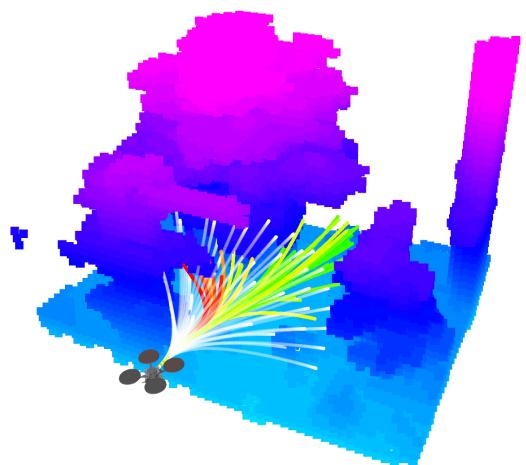
\includegraphics[width=\linewidth]{figures/01_anchor_exploration.jpg}
      \begin{center}
      \scriptsize\color{yopogray}
      原文 Fig.~1：运动基元（白线）作为锚点铺满解空间；\\
      按评分着色的预测曲线为优化结果
      \end{center}
    \end{column}
  \end{columns}
\end{frame}

\begin{frame}{方法概述：单次前向传播的规划流程}
  \begin{columns}[c]
    \begin{column}{0.6\textwidth}
      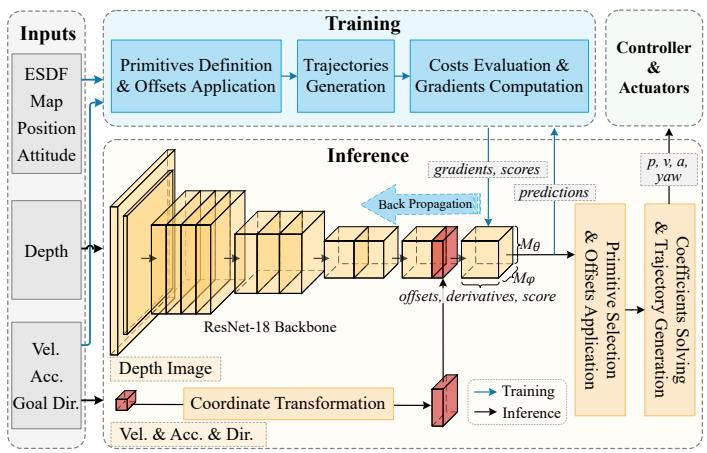
\includegraphics[width=\linewidth]{figures/03_system_overview.jpg}
      \begin{center}\scriptsize\color{yopogray}
      原文 Fig.~3：深度图 + 当前状态 + 目标方向 $\to$ 每个基元的
      偏移、终端导数、评分；\textbf{训练时}由 ESDF 计算代价与梯度
      \end{center}
    \end{column}
    \begin{column}{0.38\textwidth}
      \small
      \begin{itemize}\tight
        \item 感知 $\to$ ResNet-18 主干
        \item 前端 $\to$ 15 个基元锚点（\textbf{预定义、不占算力}）
        \item 后端 $\to$ 网络预测的终端状态
              $+$ 五次多项式解析求解
      \end{itemize}
      \begin{reading}
        \scriptsize
        图上“Training / Inference”两条支路共用同一个网络：
        差别在于训练阶段增加了查询地图并计算梯度的评价环节。
      \end{reading}
    \end{column}
  \end{columns}
\end{frame}

\begin{frame}{坐标系定义与符号约定}
  \small
  \begin{columns}[t]
    \begin{column}{0.5\textwidth}
      \begin{block}{两个坐标系}
        \begin{itemize}\tight
          \item \textbf{机体系（body frame）}：网络输入/输出与轨迹表示所在系。
                用机体系可避免网络输出位置与姿态（降维）。
          \item \textbf{基元系（primitive frame）}：第 $(i,j)$ 个锚点自己的坐标系。
                \textbf{只用于把状态与终端导数“本地化”}，不改变物理量。
        \end{itemize}
      \end{block}
    \end{column}
    \begin{column}{0.46\textwidth}
      \begin{block}{符号速查}
        \scriptsize
        \begin{tabular}{@{}ll@{}}
          \toprule
          $D$ & 深度图 \\
          $\hat{\mathbf g}$ & 网络输入的目标单位方向 \\
          $\mathbf g_{\mathrm{local}}$ & 代价里的临时目标点 \\
          $(r,\theta_j,\varphi_i)$ & 基元球坐标参数 \\
          $\mathbf y^{\mathrm{traj}}$ & 9 维原始轨迹输出 \\
          $\mathbf q$ & 解码后的终端状态 $\mathbf p_T,\mathbf v_T,\mathbf a_T$ \\
          $\hat s$ / $J$ & 预测评分 / 外部计算的代价 \\
          $\mathbf c_\mu$, $M(T)$ & 单轴多项式系数、边界映射矩阵 \\
          \bottomrule
        \end{tabular}
      \end{block}
    \end{column}
  \end{columns}

  \begin{reading}[维度约定的统一]
    \small
    本报告图像尺寸记为“宽 $\times$ 高”，张量采用 NCHW 布局。
    原文的 $M_\varphi\times M_\theta\times 10=5\times3\times10$
    按“水平、竖直、通道”排列，对应同样的 15 个候选。
  \end{reading}
\end{frame}

% ============================ 01 前向推理 ============================

\section{前向推理：候选轨迹的生成}

\begin{frame}[plain]
  \begin{center}
    \vspace{1.2cm}
    {\color{yopoblue}\Huge\bfseries 01}\\[0.5em]
    {\color{yopoblue}\LARGE 前向推理：候选轨迹的生成}\\[1.2em]
    \begin{minipage}{0.72\textwidth}
      \small\color{yopogray}
      候选轨迹由\textbf{固定锚点}、\textbf{网络预测的有界修正量}与\textbf{五次多项式解析解}共同构成。
      网络仅输出其中的修正量与终端导数，不直接输出曲线。
    \end{minipage}
  \end{center}
\end{frame}

% ---------------------------------------------------------------
\begin{frame}[shrink=12]{规划的多模态性与多候选结构}
  \noindent
  \begin{minipage}[t]{0.4\textwidth}\vspace{0pt}
      \scriptsize
      \begin{block}{问题}
        \begin{itemize}\tight
          \item 左绕、右绕都可行，都存在合理解；
          \item 单一回归头把它压成一个输出 $\Rightarrow$ \textbf{折中解}；
          \item 多假设 + winner-takes-all $\Rightarrow$ \textbf{模式坍缩}。
        \end{itemize}
      \end{block}
  \end{minipage}\hfill
  \begin{minipage}[t]{0.57\textwidth}\vspace{0pt}
      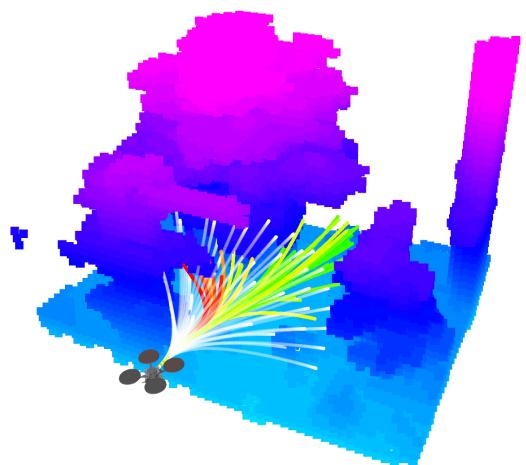
\includegraphics[width=0.74\linewidth]{figures/01_anchor_exploration.jpg}
      \begin{center}\scriptsize\color{yopogray}
      原文 Fig.~1：白线为运动基元锚点，\\
      彩色曲线为按评分着色的预测结果
      \end{center}
  \end{minipage}
  \begin{paperfinding}[原文的解法]
    \scriptsize
    借鉴 YOLO 的“\textbf{锚框 + 偏移}”结构：
    在相机视场内均匀铺开一组运动基元作为\textbf{锚点}，
    让每个输出位置只负责自己那片局部解空间，
    再预测该候选的\textbf{改进量}与\textbf{质量}。
  \end{paperfinding}
\end{frame}

% ---------------------------------------------------------------
\begin{frame}{运动基元锚点的球坐标定义}
  \small
  \begin{columns}[t]
    \begin{column}{0.54\textwidth}
      以本轮规划开始时的机体坐标系表示，第 $(i,j)$ 个锚点为（原文式 (3)）：
      \[
        \mathbf p_{ij}=\bigl(r\cos\theta_j\cos\varphi_i,\;
        r\cos\theta_j\sin\varphi_i,\; r\sin\theta_j\bigr)
      \]
      \begin{itemize}\tight
        \item $\varphi_i$：水平方位角，共 $M_\varphi$ 个；
        \item $\theta_j$：竖直方向角，共 $M_\theta$ 个；
        \item $r$：基准规划半径（对应规划时域）。
      \end{itemize}
      \begin{reading}[基元库的表达空间]
        \scriptsize
        原文明确：基元库定义在 \textbf{state lattice space} 而不是多项式系数空间。
        这样表达是“\textbf{空间分离}”的——每个候选占一块位置，
        才能与卷积特征图的每个格子一一对上。
      \end{reading}
    \end{column}
    \begin{column}{0.42\textwidth}
      \begin{block}{论文实验配置}
        \scriptsize
        \begin{tabular}{@{}ll@{}}
          \toprule
          水平数 $M_\varphi$ & 5 \\
          竖直数 $M_\theta$ & 3 \\
          候选总数 & $\mathbf{15}$ \\
          相机视场（配置） & $90^\circ\times60^\circ$ \\
          图像分辨率 & $160\times96$ \\
          基准半径 $r$（配置） & 4\,m \\
          \bottomrule
        \end{tabular}
      \end{block}
      \begin{reading}
        \scriptsize
        “15 个”是\textbf{实验配置}，不是方法要求的固定常数。
        候选数由图像分辨率与下采样倍数共同决定。
      \end{reading}
    \end{column}
  \end{columns}
\end{frame}

% ---------------------------------------------------------------
\begin{frame}[shrink=12]{锚点的具体取值}
  \noindent
  \begin{minipage}[t]{0.55\textwidth}\vspace{0pt}
      \begin{block}{均匀采样 $\Rightarrow$ 具体角度}
        \scriptsize
        \textbf{水平}：步长 $90^\circ/5=18^\circ$，取 5 个格子中心
        \[
          \varphi_i \in \{-36^\circ,-18^\circ,\;0^\circ,+18^\circ,+36^\circ\}
        \]
        \textbf{竖直}：步长 $60^\circ/3=20^\circ$，取 3 个格子中心
        $\theta_j \in \{-20^\circ,\;0^\circ,+20^\circ\}$。\\
        每个锚点半径 $r=4$\,m，共 $5\times3=15$ 个锚点。
      \end{block}
  \end{minipage}\hfill
  \begin{minipage}[t]{0.41\textwidth}\vspace{0pt}
      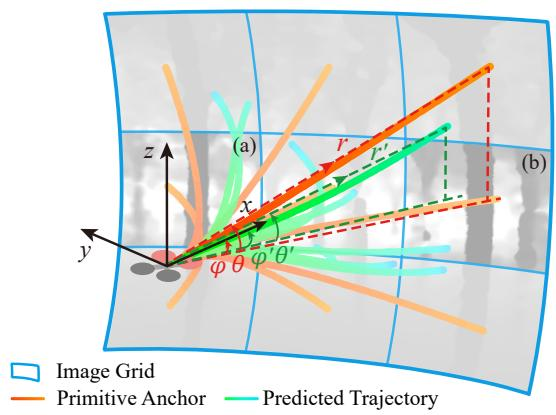
\includegraphics[width=0.9\linewidth]{figures/04_primitive_definition.jpg}
      \begin{center}\scriptsize\color{yopogray}
      原文 Fig.~4：深度图被划分为 $M_\varphi\times M_\theta$ 个格子，
      每个格子对应视锥内的一个基元
      \end{center}
  \end{minipage}
  \begin{reading}[数值来源]
    \scriptsize
    $\pm36^\circ/\pm20^\circ$ 由原文“在传感器可见范围内均匀采样”
    $+$ $5\times3$ 网格 $+$ 配置视场 $90^\circ\times60^\circ$ 推出；
    视场角与半径取自作者开源配置，论文正文只给出相机型号与图像分辨率。
  \end{reading}
\end{frame}

% ---------------------------------------------------------------
\begin{frame}{网络输出：锚点的有界修正量}
  \small
  \begin{columns}[t]
    \begin{column}{0.52\textwidth}
      对每个锚点，网络输出 3 个偏移量，用 $\tanh$ 夹在有界范围内（原文式 (8)）：
      \[
        \begin{aligned}
          \Delta\theta &= \tanh(y_\theta)\,d_\theta\\
          \Delta\varphi &= \tanh(y_\varphi)\,d_\varphi\\
          \Delta r &= \tanh(y_r)\,d_r
        \end{aligned}
      \]
      修正后的终端位置（原文式 (4)）：
      \[
        r'=r+\Delta r,\quad \varphi'=\varphi_i+\Delta\varphi,\quad \theta'=\theta_j+\Delta\theta
      \]
      再代回同一套球坐标变换得到 $\mathbf p_T$。
    \end{column}
    \begin{column}{0.44\textwidth}
      \begin{block}{偏移窗口 vs 格子大小}
        \footnotesize
        \begin{tabular}{@{}lcc@{}}
          \toprule
          方向 & 格子间距 & 偏移窗口（配置） \\
          \midrule
          水平 & $18^\circ$ & $\pm15^\circ$（共 $30^\circ$）\\
          竖直 & $20^\circ$ & $\pm15^\circ$（共 $30^\circ$）\\
          半径 & $r=4$\,m & $\pm4$\,m $\Rightarrow r'\in[0,8]$ \\
          \bottomrule
        \end{tabular}
      \end{block}
      \begin{paperfinding}[关键设计：窗口略大于格子]
        \footnotesize
        原文：“局部解空间先验\textbf{略大于}格子的视场”，
        因此相邻候选的区域可以\textbf{重叠}——
        这既保证候选互相分散（多模态），又不让它们完全无法协调。
      \end{paperfinding}
    \end{column}
  \end{columns}
\end{frame}

% ---------------------------------------------------------------
\begin{frame}{锚点可达域：球面格点与单个扇区}
  \begin{center}
    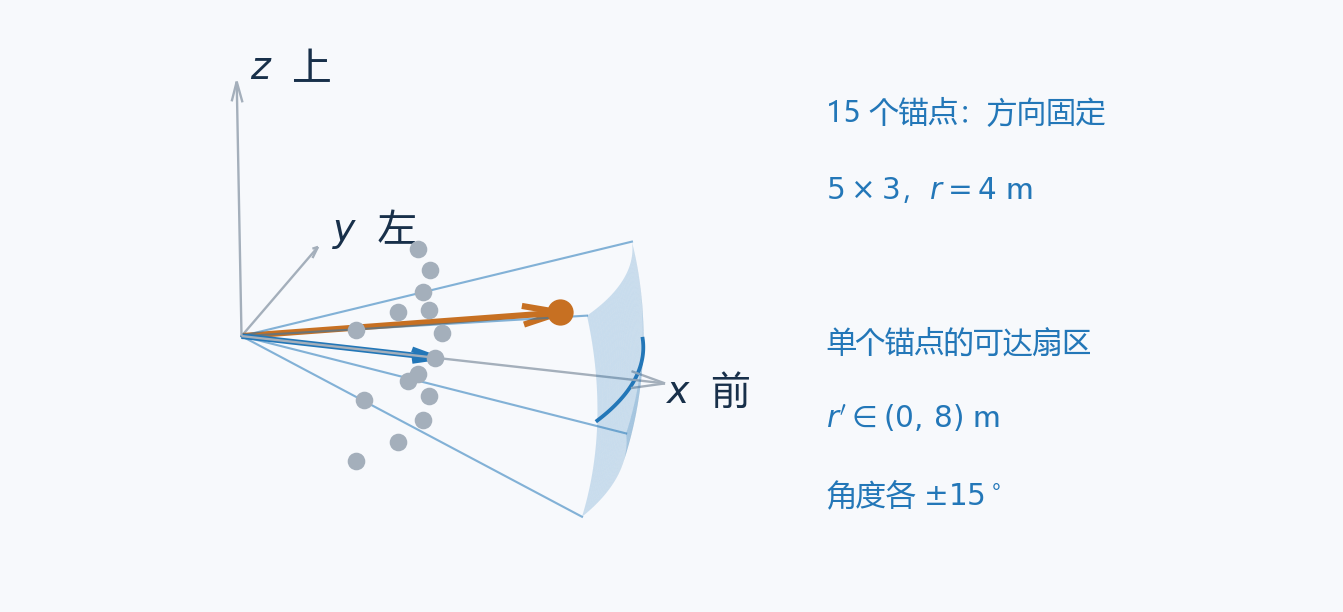
\includegraphics[width=\linewidth]{figures/24a_primitive_sector.png}
  \end{center}
\end{frame}

% ---------------------------------------------------------------
\begin{frame}{水平剖面：角度窗口与半径修正}
  \begin{center}
    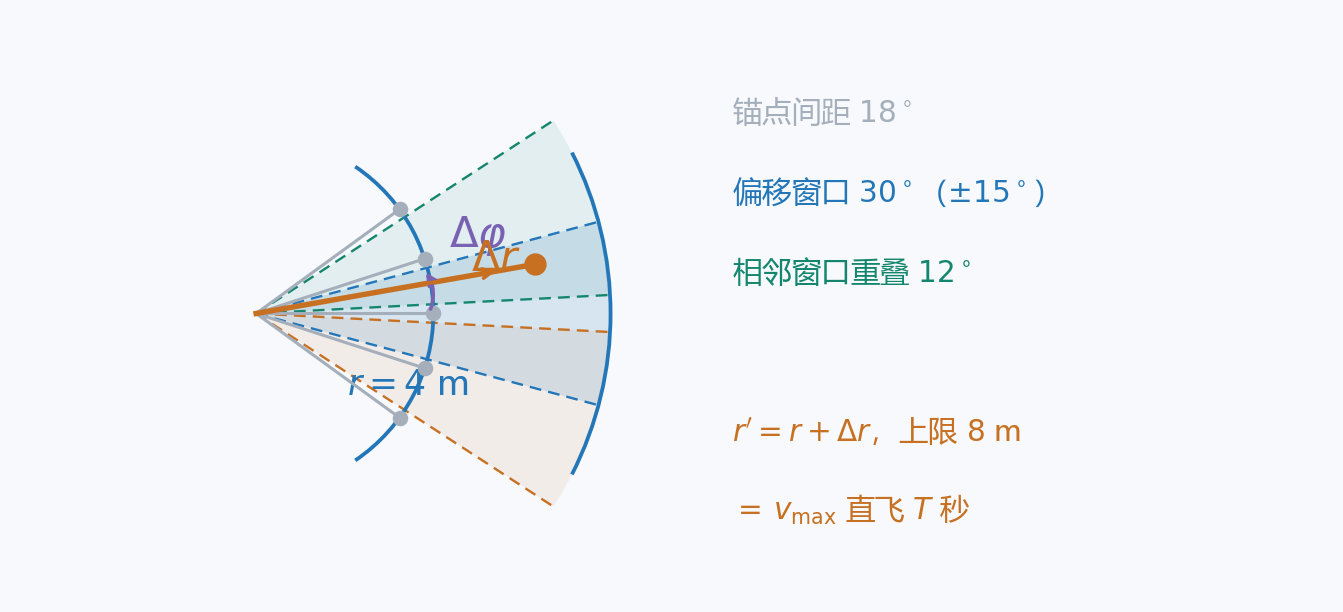
\includegraphics[width=\linewidth]{figures/24b_primitive_section.png}
  \end{center}
\end{frame}

% ---------------------------------------------------------------
\begin{frame}{基元坐标系与机体坐标系的变换关系}
  \begin{center}
    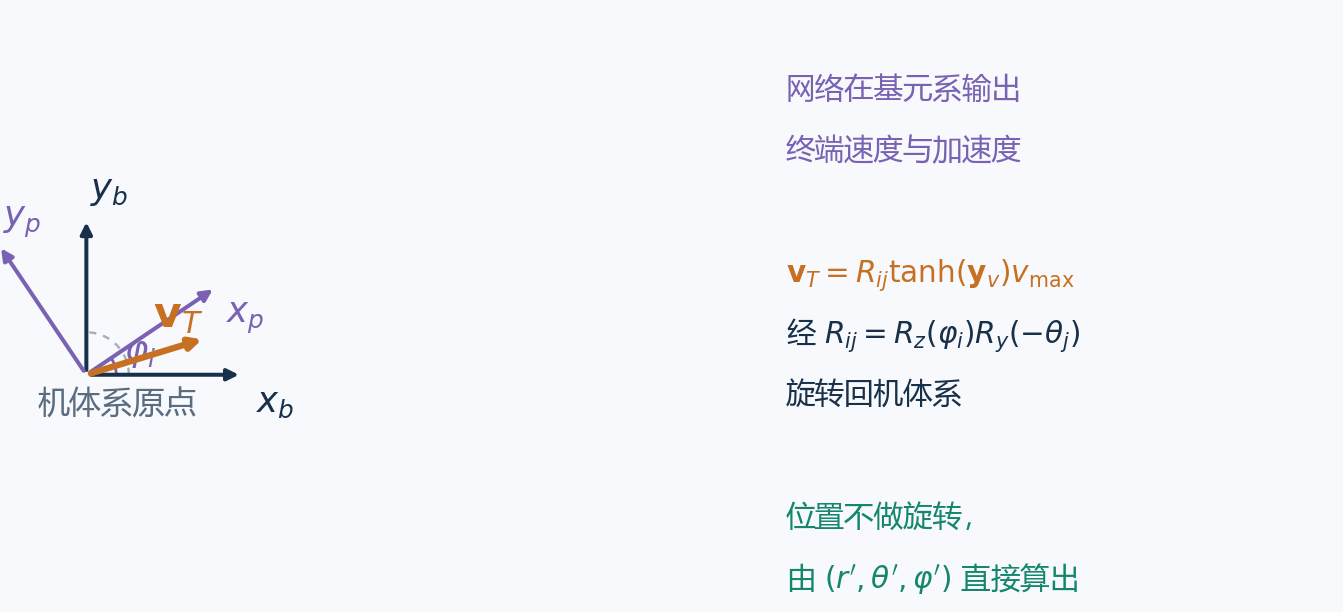
\includegraphics[width=\linewidth]{figures/24c_frame_rotation.png}
  \end{center}
\end{frame}

% ---------------------------------------------------------------
\begin{frame}[shrink=6]{终端速度与加速度的预测}
  \small
  \begin{columns}[t]
    \begin{column}{0.5\textwidth}
      \small
      终端导数同样经 $\tanh$ 限幅，再从基元系转回机体系（原文式 (9)）：
      \[
        \begin{aligned}
          \mathbf v_T &= R_{ij}\,\tanh(\mathbf y_v)\,v_{\max}\\
          \mathbf a_T &= R_{ij}\,\tanh(\mathbf y_a)\,a_{\max}
        \end{aligned}
      \]
      \begin{itemize}\tight
        \item $R_{ij}$：基元系 $\to$ 机体系的旋转（式 (6)）；
        \item 限幅的目的：\textbf{动力学可行}——
              终端速度/加速度不会超出训练分布。
      \end{itemize}
    \end{column}
    \begin{column}{0.46\textwidth}
      \begin{reading}[终端状态的信息量]
        \scriptsize
        终点位置相同、终端速度/加速度不同，整条曲线的形状仍然不同。
        所以网络输出的 9 个数比“一个目标点”信息量大得多，
        它同时表达了\textbf{靠近的方式}。
      \end{reading}
      \begin{reading}[限幅的作用范围]
        \scriptsize
        对\textbf{输出分量}限幅，不能直接解释为对整条轨迹的速度模长、
        推力或角速度的严格保证。
      \end{reading}
    \end{column}
  \end{columns}
\end{frame}

% ---------------------------------------------------------------
\begin{frame}{网络结构：ResNet-18 主干 + 共享 $1\times1$ 卷积头}
  \small
  \begin{columns}[t]
    \begin{column}{0.55\textwidth}
      \begin{block}{张量形状流（批次 $B$）}
        \scriptsize
        \begin{tabular}{@{}lll@{}}
          \toprule
          数据 & 形状 & 说明 \\
          \midrule
          深度图 & $B{\times}1{\times}96{\times}160$ & 单通道深度 \\
          图像特征 & $B{\times}64{\times}3{\times}5$ & ResNet-18，32 倍下采样 \\
          状态张量 & $B{\times}9{\times}3{\times}5$ & 每个基元一份坐标变换 \\
          头输入 & $B{\times}73{\times}3{\times}5$ & $64+9$ 通道拼接 \\
          原始输出 & $B{\times}10{\times}3{\times}5$ & 每个格子 10 个数 \\
          可重排为 & $B{\times}15{\times}10$ & 15 组“9 参数 + 1 评分” \\
          \bottomrule
        \end{tabular}
      \end{block}
    \end{column}
    \begin{column}{0.41\textwidth}
      \begin{itemize}\tight
        \item 主干是\textbf{改过的 ResNet-18}：单通道输入、
              去掉平均池化、$1\times1$ 卷积输出 64 通道特征图；
        \item 预测头是三层 $1\times1$ 卷积（256–256–10），\textbf{权重共享}；
        \item 状态分支是一个\textbf{空的 Sequential}——
              状态几乎只做几何处理，不经过额外网络层。
      \end{itemize}
      \begin{reading}
        \scriptsize
        15 个候选是\textbf{一次张量计算}并行产出的：
        共享骨干张量上的不同空间位置，
        不是 15 个线程或 15 个独立网络。
      \end{reading}
    \end{column}
  \end{columns}
\end{frame}

% ---------------------------------------------------------------
\begin{frame}{特征图网格与运动基元的空间对应}
  \small
  \begin{columns}[t]
    \begin{column}{0.52\textwidth}
      \begin{block}{几何上的对应关系}
        \footnotesize
        下采样 32 倍：$96\times160 \longrightarrow 3\times5$。
        特征图的 \textbf{3 行 = 竖直 3 个基元}，
        \textbf{5 列 = 水平 5 个基元}——格子与锚点一一对应。
      \end{block}
      \begin{reading}[必须澄清的一点]
        \small
        对应关系是\textbf{位置级}的，不是“信息隔离”的：
        卷积感受野覆盖整张图，
        \textbf{每个格子看到的是全局上下文的特征}，
        而不是自己视锥那一小块。
      \end{reading}
    \end{column}
    \begin{column}{0.44\textwidth}
      \begin{block}{与图像格子编号的错位}
        \footnotesize
        格子的行优先展开顺序与基元的极坐标索引顺序\textbf{相反}
        （图像从左到右、从下到上，而基元按另一顺序编号），
        实现时需要一次索引翻转：
        \[
          \text{grid} \;\leftrightarrow\; \text{lattice}=14-\text{grid}
        \]
        这只影响实现，不改变物理含义。
      \end{block}
    \end{column}
  \end{columns}
\end{frame}

% ---------------------------------------------------------------
\begin{frame}{基元坐标系：规划问题的非平移不变性}
  \small
  \begin{columns}[t]
    \begin{column}{0.5\textwidth}
      原文式 (6)：机体 $\to$ 基元的旋转
      \[
        R_{ij}=R_z(\varphi_i)R_y(-\theta_j)
      \]
      原文式 (7)：输入状态变换到基元系
      \[
        \mathbf x'_{ij}=R_{ij}^{-1}\mathbf x
      \]
      $R_{ij}$ 的直观含义：
      “把机体系下的状态，表达成\textbf{相对于这个候选方向}的量”。
    \end{column}
    \begin{column}{0.46\textwidth}
      \begin{paperfinding}[矛盾在哪里]
        \small
        图 4 中，左侧格子 (a) 需要“向右”的偏移，
        右侧格子 (b) 需要“向左”的偏移——
        \textbf{同样的特征，期望的输出相反}。
        共享权重的卷积头无法同时满足，
        除非输入被表达成“相对量”。
      \end{paperfinding}
      \begin{reading}
        \scriptsize
        这正是 $1\times1$ 卷积共享权重能成立的前提：
        不是让网络学会 15 套规则，而是把 15 个问题\textbf{归一化成同一个问题}。
      \end{reading}
    \end{column}
  \end{columns}
\end{frame}

% ---------------------------------------------------------------
\begin{frame}{状态输入的构造与坐标变换}
  \small
  \begin{columns}[t]
    \begin{column}{0.54\textwidth}
      \begin{block}{输入状态的构造}
        \footnotesize
        \begin{itemize}\tight
          \item 机体系 9 维状态：速度(3) + 加速度(3) + 目标单位方向(3)；
          \item 归一化：$\mathbf v/v_{\max}$、$\mathbf a/a_{\max}$、
                目标方向单位化并设下限（避免除零）；
          \item 对每个基元旋转一次：
                $\mathbf x'_{ij}=[\;R_{ij}^{-1}\mathbf v,\;R_{ij}^{-1}\mathbf a,\;R_{ij}^{-1}\hat{\mathbf g}\;]$
          \item 得到 $B\times9\times3\times5$，与图像特征\textbf{按通道拼接}。
        \end{itemize}
      \end{block}
    \end{column}
    \begin{column}{0.42\textwidth}
      \begin{reading}[实现上的常见错误]
        \small
        9 维状态是\textbf{三个 3 维向量}，需分别旋转；
        不能用一个 $3\times3$ 矩阵去乘 $9\times1$ 的向量。
        等价写法是块对角矩阵
        $\operatorname{diag}(R^{-1},R^{-1},R^{-1})$。
      \end{reading}
      \begin{reading}[方向约定]
        \scriptsize
        按原文式 (7)(9)：机体系向量转到基元系用 $R_{ij}^{-1}$，
        基元系终端导数转回机体系用 $R_{ij}$。
        实现时应依此核对方向，避免仅凭矩阵名称判断。
      \end{reading}
    \end{column}
  \end{columns}
\end{frame}

% ---------------------------------------------------------------
\begin{frame}{候选输出参数：每组 10 个分量}
  \small
  \begin{columns}[t]
    \begin{column}{0.5\textwidth}
      第 $i$ 个候选的原始输出向量：
      \[
        \mathbf y_i=\bigl[y_\theta,\;y_\varphi,\;y_r,\;
        \mathbf y_v^{\mathsf T},\;\mathbf y_a^{\mathsf T},\;\hat s_i\bigr]^{\mathsf T}
      \]
      前 9 个经偏移、限幅与旋转，得到有物理意义的终端状态：
      \[
        \mathbf q_i=\bigl[\mathbf p_{T,i}^{\mathsf T},\;
        \mathbf v_{T,i}^{\mathsf T},\;\mathbf a_{T,i}^{\mathsf T}\bigr]^{\mathsf T}\in\mathbb R^9
      \]
      第 10 个 $\hat s_i$ 是\textbf{该候选的代价估计}（评分）。
    \end{column}
    \begin{column}{0.46\textwidth}
      \begin{block}{10 个输出的分工}
        \footnotesize
        \begin{tabular}{@{}cll@{}}
          \toprule
          序号 & 含义 & 解码 \\
          \midrule
          1 & 方位角偏移 & $\tanh\cdot15^\circ$ \\
          2 & 俯仰角偏移 & $\tanh\cdot15^\circ$ \\
          3 & 半径偏移 & $\tanh\cdot r$ \\
          4--6 & 终端速度 & $R\tanh\cdot v_{\max}$ \\
          7--9 & 终端加速度 & $R\tanh\cdot a_{\max}$ \\
          10 & 评分 & 单调激活 \\
          \bottomrule
        \end{tabular}
      \end{block}
      \begin{reading}
        \scriptsize
        评分与轨迹参数从\textbf{同一组共享特征}中同时产生；
        评分不是另一个“接收完整曲线、在线查地图”的独立评价网络。
      \end{reading}
    \end{column}
  \end{columns}
\end{frame}

% ---------------------------------------------------------------
\begin{frame}{从终端状态到连续曲线：五次多项式边界值问题}
  \small
  \begin{columns}[t]
    \begin{column}{0.52\textwidth}
      对任一轴 $\mu\in\{x,y,z\}$（原文式 (1)(2)(5)）：
      \[
        p_\mu(t)=c_0+c_1t+c_2t^2+c_3t^3+c_4t^4+c_5t^5
      \]
      把\textbf{当前状态}与\textbf{终端状态}组成边界向量 $\mathbf d$，
      用常数矩阵映射到系数（原文式 (5)）：
      \[
        \mathbf c_\mu = M(T)^{-1}\mathbf d_\mu
      \]
      \[
        M(T)=
        \begin{bmatrix}
          1&0&0&0&0&0\\
          0&1&0&0&0&0\\
          0&0&2&0&0&0\\
          1&T&T^2&T^3&T^4&T^5\\
          0&1&2T&3T^2&4T^3&5T^4\\
          0&0&2&6T&12T^2&20T^3
        \end{bmatrix}
      \]
    \end{column}
    \begin{column}{0.44\textwidth}
      \begin{block}{六个边界条件}
        \footnotesize
        起点：位置 $\mathbf p_0$、速度 $\mathbf v_0$、加速度 $\mathbf a_0$\\
        终点：位置 $\mathbf p_T$、速度 $\mathbf v_T$、加速度 $\mathbf a_T$
      \end{block}
      \begin{reading}[三个轴各解一次]
        \small
        三个轴分别求解，共 18 个系数。
        $T>0$ 时矩阵可逆、解唯一，且固定 $T$ 后可\textbf{预先算好} $M(T)^{-1}$——
        在线求解只是几次矩阵乘。
      \end{reading}
      \begin{reading}[不提供什么保证]
        \scriptsize
        单段多项式保证连续可导并精确满足边界条件，
        \textbf{不自动保证无碰撞}或满足全部动力学硬约束。
      \end{reading}
    \end{column}
  \end{columns}
\end{frame}

% ---------------------------------------------------------------
\begin{frame}{在线推理流程}
  \begin{columns}[c]
    \begin{column}{0.55\textwidth}
      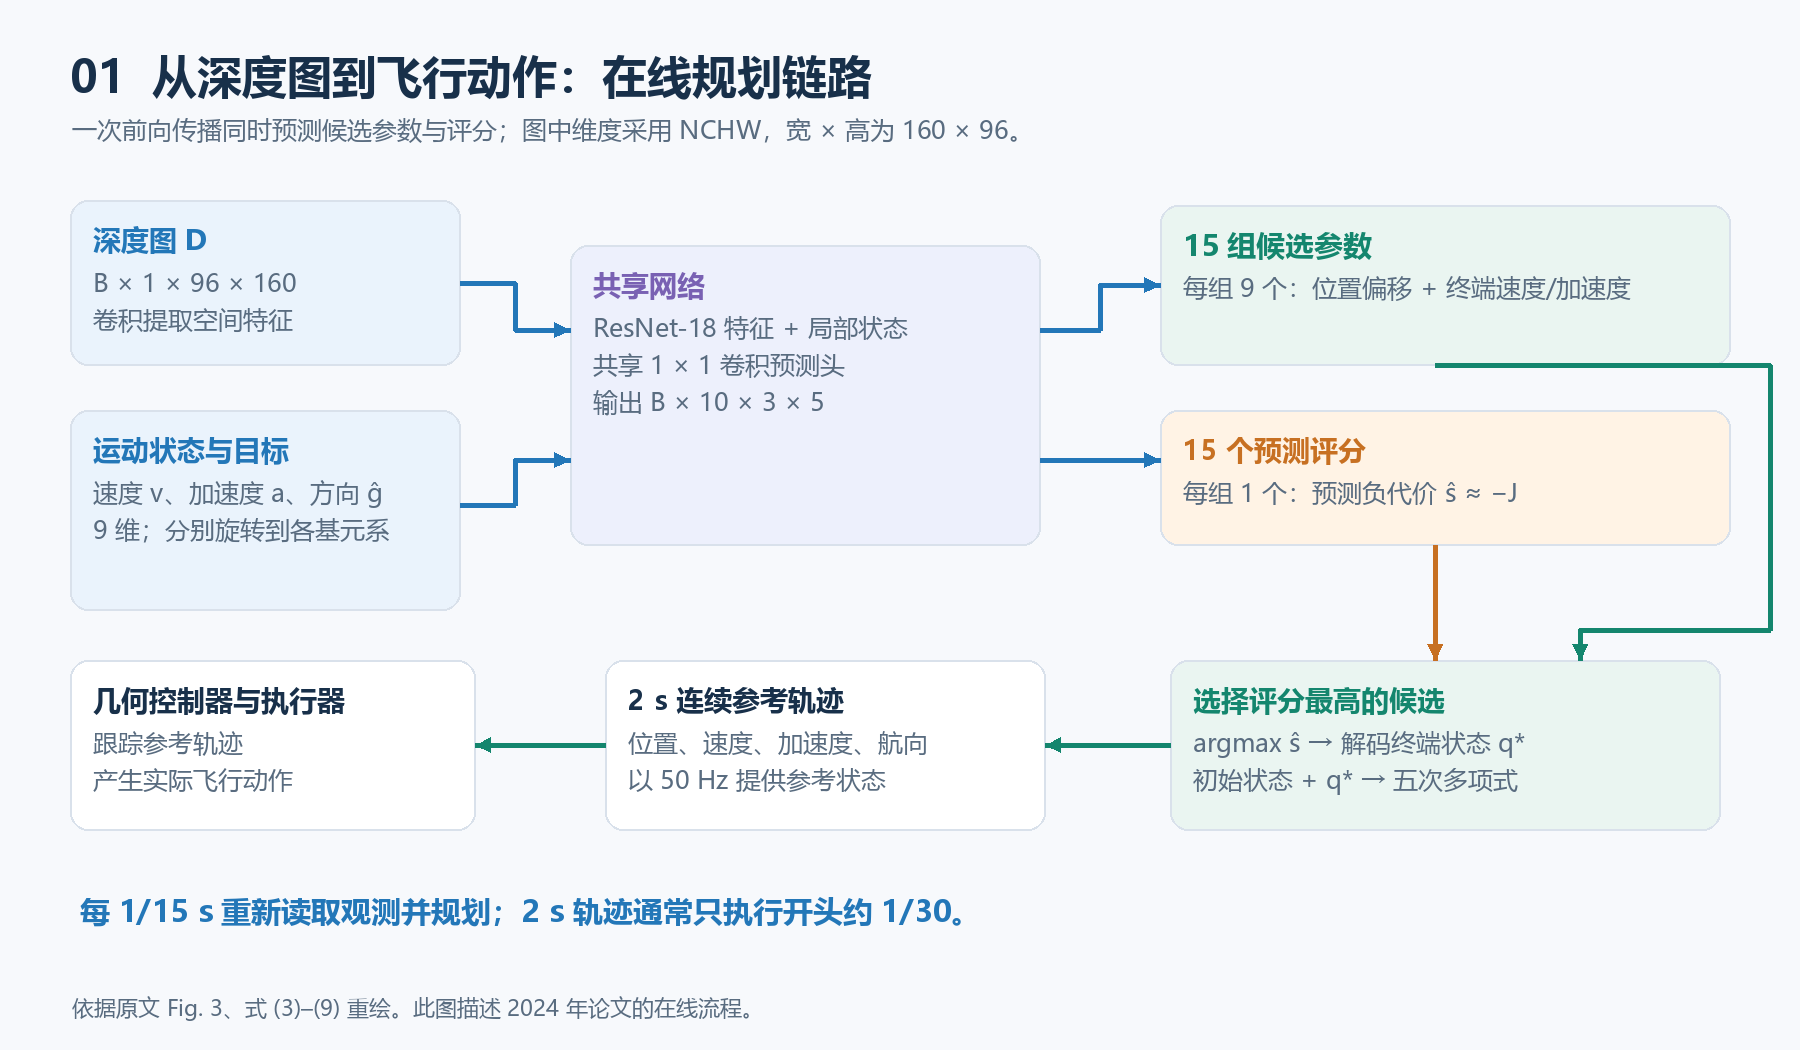
\includegraphics[width=\linewidth]{figures/20_note_online_pipeline.png}
    \end{column}
    \begin{column}{0.43\textwidth}
      \small
      \footnotesize
      \begin{enumerate}\tight
        \item 取深度图 + 当前速度、加速度、目标方向；
        \item 提特征、把状态变换到各基元系并拼接；
        \item 共享头同时输出 \textbf{15 组轨迹参数 + 15 个评分}；
        \item 选\textbf{评分最好}的候选，解码其终端状态；
        \item 代入边界值问题，求出五次多项式；
        \item 输出参考位置、速度、加速度、航向给控制器。
      \end{enumerate}
      \begin{paperfinding}[算力上的关键]
        \scriptsize
        在线\textbf{只对选中的那条轨迹求解多项式}；
        另外 14 条只是网络输出，不进入求解、不查地图。
      \end{paperfinding}
    \end{column}
  \end{columns}
\end{frame}

% ---------------------------------------------------------------
\begin{frame}{规划与控制的时序关系}
  \small
  \begin{center}
  \begin{tikzpicture}[x=1cm,y=1cm,every node/.style={font=\small}]
    \draw[->,thick,yopoblue] (0,0) -- (11,0) node[anchor=west,font=\footnotesize]{时间};
    \foreach \x/\lab in {0/0,2.5/0.5,5/1.0,7.5/1.5,10/2.0}
      \draw[yopoblue] (\x,0.08) -- (\x,-0.08) node[below,font=\scriptsize]{\lab\,s};
    \draw[very thick,yopoorange] (0,0.35) -- (3,0.35);
    \draw[very thick,yopogreen]  (0,0.75) -- (2.5,0.75);
    \node[anchor=west,font=\scriptsize,color=yopoorange] at (3.05,0.35) {重规划周期 $1/15$\,s（15\,Hz）};
    \node[anchor=west,font=\scriptsize,color=yopogreen]  at (2.55,0.75) {执行 $1/30$ 段（约 66.7\,ms）};
    \draw[decorate,decoration={brace,amplitude=5pt},yopoblue] (0,-0.35) -- (10,-0.35)
      node[midway,below=4pt,font=\scriptsize,color=yopoblue]{规划窗口 $T=2$\,s};
  \end{tikzpicture}
  \end{center}
  \vspace{-0.3em}
  \begin{columns}[t]
    \begin{column}{0.48\textwidth}
      \begin{paperfinding}[原文给出的三个数]
        \footnotesize
        \begin{itemize}\tight
          \item 规划时域：$2$\,s；
          \item 重规划频率：\textbf{15\,Hz}；
          \item 参考状态输出：\textbf{50\,Hz}；
          \item 只执行一条 2\,s 轨迹开头约 $1/30$ 的部分。
        \end{itemize}
      \end{paperfinding}
    \end{column}
    \begin{column}{0.48\textwidth}
      \begin{reading}[该时序设计的依据]
        \footnotesize
        推得越远，规划的置信度越低，但推得远才能在高速下留出反应余量；
        “规划 2\,s、执行 1/30”是\textbf{滚动重规划}的典型折中。
        \textbf{“Only Plan Once”指每轮规划一次前向}，
        不等于整段飞行只规划一次。
      \end{reading}
    \end{column}
  \end{columns}
\end{frame}

% ---------------------------------------------------------------
\begin{frame}{前向推理小结：固定量与预测量}
  \small
  \begin{columns}[t]
    \begin{column}{0.5\textwidth}
      \begin{block}{配置预设（训练后不再改变）}
        \footnotesize
        \begin{tabular}{@{}ll@{}}
          \toprule
          项目 & 取值 \\
          \midrule
          基元数量与初始方向 & $5\times3$，$\pm36^\circ/\pm20^\circ$ \\
          基准半径 $r$ & 4\,m \\
          偏移上限 $d_\varphi,d_\theta,d_r$ & $15^\circ,15^\circ,4$\,m \\
          规划时域与输出缩放 & $T$、$v_{\max}$、$a_{\max}$ \\
          \bottomrule
        \end{tabular}
      \end{block}
    \end{column}
    \begin{column}{0.46\textwidth}
      \begin{block}{每次前向重新预测}
        \footnotesize
        \begin{itemize}\tight
          \item 位置偏移 $\Delta\varphi,\Delta\theta,\Delta r$；
          \item 终端速度 $\mathbf v_T$、终端加速度 $\mathbf a_T$；
          \item 每个候选的评分 $\hat s_i$。
        \end{itemize}
      \end{block}
      \begin{reading}
        \scriptsize
        “偏移上限固定”不代表“偏移值固定”：
        权重训练完成后不再变化，
        但不同观测与状态仍会产生不同输出。
      \end{reading}
    \end{column}
  \end{columns}

  \vspace{0.2em}
  \begin{teach}[流程小结]
    \small
    深度图 $\to$ 15 组“锚点 + 有界修正 + 终端导数 + 评分”
    $\to$ 选出评分最好的一组 $\to$ 与当前状态一起解五次多项式
    $\to$ 连续参考轨迹 $\to$ 控制器。
  \end{teach}
\end{frame}

% ---------------------------------------------------------------
\begin{frame}{前向推理的常见误解}
  \small
  \begin{center}
  \begin{tabular}{@{}p{0.42\textwidth}p{0.5\textwidth}@{}}
    \toprule
    \textbf{常见误解} & \textbf{准确理解} \\
    \midrule
    15 个固定动作里选一个 &
    锚点固定，但每次前向都在锚点附近\textbf{预测可变的终端状态}，再选择 \\
    \addlinespace
    15 个区域各跑一个搜索器 / 线程 &
    共享网络在\textbf{一次张量计算}中同时产生 15 个空间位置的输出 \\
    \addlinespace
    只输出 2\,s 之后的终点位置 &
    还输出终端\textbf{速度、加速度}与\textbf{评分}；三者共同决定曲线形状 \\
    \addlinespace
    网络直接输出多项式系数 &
    网络只输出\textbf{边界参数}，系数由解析映射 $M(T)^{-1}$ 得到 \\
    \addlinespace
    在线把所有候选曲线都解出来再查地图打分 &
    评分是\textbf{同时预测}的；在线只求解被选中的那条曲线 \\
    \addlinespace
    终端限幅 $\Rightarrow$ 全程安全可执行 &
    限幅与软代价改善表现，\textbf{不构成}全程硬约束证明 \\
    \bottomrule
  \end{tabular}
  \end{center}
\end{frame}

% ============================ 02 引导训练 ============================

\section{引导训练：代价梯度的传递机制}

\begin{frame}[plain]
  \begin{center}
    \vspace{1.2cm}
    {\color{yopoblue}\Huge\bfseries 02}\\[0.5em]
    {\color{yopoblue}\LARGE 引导训练：代价梯度的传递机制}\\[1.2em]
    \begin{minipage}{0.76\textwidth}
      \small\color{yopogray}
      训练阶段的评价环节并非学习得到的专家模型，而是由代价函数与特权地图查询构成的数值计算过程：
      给定候选的终端状态，返回代价 $J$ 与该终端状态的梯度；
      再由链式法则将其传递至网络权重。
    \end{minipage}
  \end{center}
\end{frame}

% ---------------------------------------------------------------
\begin{frame}{三种学习范式的比较}
  \begin{columns}[c]
    \begin{column}{0.55\textwidth}
      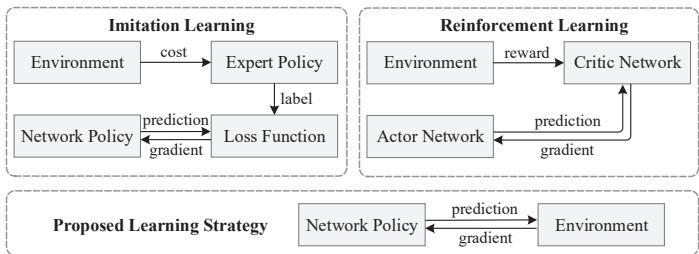
\includegraphics[width=\linewidth]{figures/02_learning_paradigms.jpg}
      \begin{center}\scriptsize\color{yopogray}
      原文 Fig.~2：模仿学习 / 强化学习 / 本文策略的对照
      \end{center}
    \end{column}
    \begin{column}{0.43\textwidth}
      \small
      \begin{itemize}\tight
        \item \textbf{模仿学习}：环境 $\to$ 专家 $\to$ 标签 $\to$ 损失；
              网络的上界就是专家。
        \item \textbf{强化学习}：环境给奖励 $\to$ 训练 Critic 来近似可导函数；
              奖励稀疏、需要大量交互。
        \item \textbf{引导学习}：环境\textbf{直接}给出可求导的代价——
              省掉中间那层近似。
      \end{itemize}
      \begin{reading}[关键区别]
        \small
        YOPO 认为规划问题的本质就是\textbf{梯度优化}。
        既然代价能求梯度，就没有必要先训一个 Critic 来假装它可导。
      \end{reading}
    \end{column}
  \end{columns}
\end{frame}

% ---------------------------------------------------------------
\begin{frame}{不同训练范式的代价分布对比}
  \small
  \begin{columns}[t]
    \begin{column}{0.6\textwidth}
      \begin{center}
      \begin{tabular}{@{}cc@{}}
        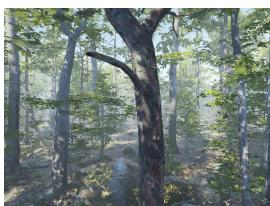
\includegraphics[width=0.36\linewidth]{figures/05a_simulated_scene.jpg} &
        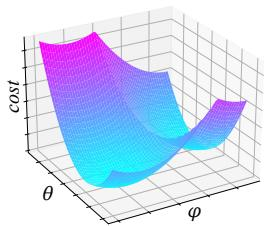
\includegraphics[width=0.36\linewidth]{figures/05b_wta_cost.jpg}\\
        \scriptsize (a) 仿真场景 &
        \scriptsize (b) Winner-Takes-All 代价 \\[3pt]
        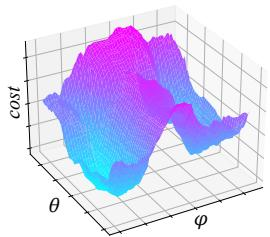
\includegraphics[width=0.36\linewidth]{figures/05c_critic_cost.jpg} &
        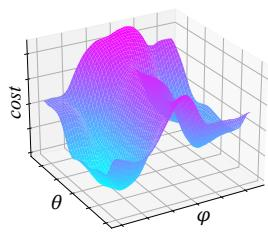
\includegraphics[width=0.36\linewidth]{figures/05d_realistic_cost.jpg}\\
        \scriptsize (c) Critic 网络给出的代价 &
        \scriptsize (d) 真实代价 \\
      \end{tabular}
      \end{center}
    \end{column}
    \begin{column}{0.38\textwidth}
      \scriptsize
      \begin{itemize}\tight
        \item \textbf{(b) 监督/模仿}：距离标签的二次型——
              一个光滑的碗，\textbf{没有多模态结构}。
        \item \textbf{(c) Critic}：训练不足时\textbf{噪声大}、曲面不平滑。
        \item \textbf{(d) 真实代价}：来自 ESDF 与运动学，
              有起伏、有多个局部极小——\textbf{这才是要拟合的目标}。
      \end{itemize}
      \begin{reading}
        \scriptsize
        原文 Fig.~5：固定当前状态、规划时域与终端导数，
        把 $\varphi,\theta$ 当自由变量画出的代价分布。
        把代价简化成“离标签多远”，信息量远不如直接使用规划代价本身。
      \end{reading}
    \end{column}
  \end{columns}
\end{frame}

% ---------------------------------------------------------------
\begin{frame}{引导学习：以数值梯度作为监督信号}
  \small
  \begin{columns}[t]
    \begin{column}{0.5\textwidth}
      \begin{block}{传统梯度优化的做法}
        \footnotesize
        查 ESDF 得到数值梯度 $\partial J/\partial(\text{轨迹参数})$，
        直接\textbf{更新轨迹参数}（多项式路点或 B 样条控制点）。
      \end{block}
      \begin{block}{YOPO 多做了一步}
        \footnotesize
        把这同一个数值梯度，\textbf{继续沿链式法则反传}
        到“生成这些轨迹参数的网络权重”。
      \end{block}
      \begin{paperfinding}[原文的三点理由]
        \footnotesize
        反馈\textbf{真实}（就是规划代价本身）、\textbf{准确}（不是近似目标）、
        \textbf{及时}（无需与环境反复交互）。
      \end{paperfinding}
    \end{column}
    \begin{column}{0.46\textwidth}
      \begin{teach}[两种更新对象的对照]
        \small
        \begin{tabular}{@{}p{0.44\linewidth}p{0.46\linewidth}@{}}
          \toprule
          传统优化器 & YOPO 训练 \\
          \midrule
          更新\newline 轨迹变量 $\mathbf q$ &
          更新\newline \textbf{生成 $\mathbf q$ 的网络权重} \\
          \addlinespace
          每条轨迹\newline 各自迭代 &
          共享权重\newline 一次反传覆盖 15 条 \\
          \addlinespace
          用最优解 & 用\textbf{代价梯度方向}，不必先给出唯一最优解 \\
          \bottomrule
        \end{tabular}
      \end{teach}
    \end{column}
  \end{columns}
\end{frame}

% ---------------------------------------------------------------
\begin{frame}{代价函数的构成}
  \small
  \begin{columns}[t]
    \begin{column}{0.5\textwidth}
      原文式 (10)：
      \[
        J=\lambda_sJ_s+\lambda_oJ_o+\lambda_gJ_g
      \]
      \begin{itemize}\tight
        \item $J_s$：平滑项，约束导数的平方积分；
        \item $J_o$：避障项，对靠近障碍施加惩罚；
        \item $J_g$：目标项，牵引朝向目标。
      \end{itemize}
      \begin{reading}[“真实代价”的含义]
        \small
        指\textbf{按设定的规划目标与训练环境直接计算}的值，
        并不是实际闭环飞行长期收益或安全性的完整真值。
      \end{reading}
    \end{column}
    \begin{column}{0.46\textwidth}
      \begin{block}{三个子问题}
        \footnotesize
        \begin{tabular}{@{}p{0.32\linewidth}p{0.6\linewidth}@{}}
          \toprule
          项 & 是否可解析求导 \\
          \midrule
          平滑 $J_s$ & \textbf{能}：轨迹是多项式，
                       代价可写成边界状态的二次型，梯度是闭式 \\
          \addlinespace
          目标 $J_g$ & \textbf{能}：终端位置的平方距离，梯度 $2(\mathbf p_T-\mathbf g)$ \\
          \addlinespace
          避障 $J_o$ & \textbf{不能}：距离来自 ESDF，
                       只能查表 + 差分，再按链式法则拼出梯度 \\
          \bottomrule
        \end{tabular}
      \end{block}
      \begin{reading}
        \scriptsize
        该区分与后文 $\partial J/\partial\mathbf q$ 的构成对应：
        三项中只有避障项依赖地图查询，因此该项梯度为数值形式。
      \end{reading}
    \end{column}
  \end{columns}
\end{frame}

% ---------------------------------------------------------------
\begin{frame}{边界状态的固定块与自由块分解}
  \small
  \begin{columns}[t]
    \begin{column}{0.52\textwidth}
      原文式 (11)：用选择矩阵 $C$ 把边界状态拆开
      \[
        \mathbf A=M^{-1}C\begin{bmatrix}\mathbf d_F\\ \mathbf d_P\end{bmatrix}
      \]
      \begin{itemize}\tight
        \item $\mathbf d_F$：\textbf{固定块}——当前状态（起点），来自状态估计，不可改；
        \item $\mathbf d_P$：\textbf{自由块}——终端状态，由网络预测，是待优化的量。
      \end{itemize}
      \begin{paperfinding}[与经典方法的差别]
        \small
        经典方法常在\textbf{固定终点}的前提下优化分段多项式；
        这里固定的是\textbf{时间 $T$}，
        优化的是\textbf{单段多项式的自由终点}。
      \end{paperfinding}
    \end{column}
    \begin{column}{0.44\textwidth}
      \begin{teach}[该拆分的意义]
        \small
        拆分之后，代价就变成“$\mathbf d_F$ 与 $\mathbf d_P$ 的二次型”，
        而网络只需要对 $\mathbf d_P$ 负责。
        于是 $\partial J/\partial\mathbf d_P$ 就是需要反传给网络的那一份梯度，
        $\partial J/\partial\mathbf d_F$ 不需要——起点不是网络产生的。
      \end{teach}
    \end{column}
  \end{columns}
\end{frame}

% ---------------------------------------------------------------
\begin{frame}{平滑项：二次型形式与解析梯度}
  \small
  \begin{columns}[t]
    \begin{column}{0.54\textwidth}
      原文式 (12)(13)：把 $\mathbf c^T M^{-T}QM^{-1}C$ 记作 $B$，则
      \[
        J_s=
        \begin{bmatrix}\mathbf d_F\\ \mathbf d_P\end{bmatrix}^{\!\mathsf T}
        \begin{bmatrix}B_{FF}&B_{FP}\\ B_{PF}&B_{PP}\end{bmatrix}
        \begin{bmatrix}\mathbf d_F\\ \mathbf d_P\end{bmatrix}
      \]
      原文式 (14)：对自由块求导
      \[
        \frac{\partial J_s}{\partial\mathbf d_P}
        =2\,\mathbf d_F^{\mathsf T}B_{FP}+2\,\mathbf d_P^{\mathsf T}B_{PP}
      \]
      \begin{reading}[闭式梯度的来源]
        \scriptsize
        轨迹参数对边界条件是\textbf{线性}的（$\mathbf c=M^{-1}\mathbf d$），
        而导数的平方积分对系数是\textbf{二次}的。
        线性变换代入二次型 $\Rightarrow$ 对边界条件仍是二次型，
        梯度自然是线性表达式。
      \end{reading}
    \end{column}
    \begin{column}{0.42\textwidth}
      \begin{block}{矩阵的角色}
        \footnotesize
        \begin{tabular}{@{}ll@{}}
          \toprule
          $M^{-1}$ & 边界条件 $\to$ 多项式系数 \\
          $Q$ & 导数平方积分的二次型核 \\
          $C$ & 选出自由块 \\
          $B$ & 合成后的“代价矩阵” \\
          \bottomrule
        \end{tabular}
      \end{block}
      \begin{reading}[用哪一阶导数]
        \small
        原文实验采用\textbf{ jerk（三阶导）平方的积分}衡量平滑性，
        与论文对平滑度的定义一致。
        具体阶次、权重与归一化仍应对照所引用的版本。
      \end{reading}
    \end{column}
  \end{columns}
\end{frame}

% ---------------------------------------------------------------
\begin{frame}{避障项：势函数与时间积分}
  \small
  \begin{columns}[t]
    \begin{column}{0.5\textwidth}
      原文式 (15)：把安全代价定义为势函数沿轨迹的\textbf{时间积分}，
      并离散化求和
      \[
        J_o=\int_0^{T}c(\mathbf p(t))\,dt
        \;\approx\;\sum_{\kappa=0}^{T/\delta t}c(\mathbf p(\mathcal T_\kappa))\,\delta t
      \]
      原文式 (16)：势函数取指数形式
      \[
        c(d_t)=\exp\!\Bigl(-\frac{d_t-d_0}{k}\Bigr)
      \]
      $d_t$ 为最近障碍距离，$d_0,k$ 为预设尺度参数。
    \end{column}
    \begin{column}{0.46\textwidth}
      \begin{center}
      \begin{tikzpicture}[x=0.9cm,y=0.55cm,every node/.style={font=\scriptsize}]
        \draw[->] (0,0) -- (4.6,0) node[right]{距离 $d_t$};
        \draw[->] (0,0) -- (0,2.6) node[above]{$c(d_t)$};
        \draw[thick,yopoorange,domain=0:4.4,samples=60] plot (\x,{2.3*exp(-(\x-0.6)/0.9)});
        \draw[dashed,yopogray] (0.6,0) -- (0.6,2.3);
        \node[below,color=yopogray] at (0.6,0) {$d_0$};
        \node[color=yopoorange] at (3.2,1.1) {离障碍越近，代价越大};
      \end{tikzpicture}
      \end{center}
      \vspace{-0.4em}
      \begin{paperfinding}[采用时间积分的理由]
        \footnotesize
        若用线积分，无人机会通过\textbf{缩短路程}来降低累计代价，产生“抄近道穿过障碍”的偏差。
        固定时间、自由终点的设置下，时间积分消除了这个偏差。
      \end{paperfinding}
    \end{column}
  \end{columns}
\end{frame}

% ---------------------------------------------------------------
\begin{frame}{避障项：梯度计算}
  \small
  \begin{columns}[t]
    \begin{column}{0.52\textwidth}
      原文式 (17)：离散形式的雅可比
      \[
        \frac{\partial J_o}{\partial\mathbf d_{P\mu}}
        =\sum_{\kappa=0}^{T/\delta t}
        \nabla_\mu c\bigl(\mathbf p(\mathcal T_\kappa)\bigr)\,
        \mathbf T\,\mathbf L_P\,\delta t
      \]
      该式即标准的链式相乘，两项分别对应：

      \vspace{0.3em}
      \begin{center}
      \begin{tikzpicture}[node distance=4mm,every node/.style={font=\scriptsize,align=center}]
        \node[draw=yopogreen,fill=yopopale,rounded corners,inner sep=3pt] (p) {采样点位置\\$\partial\mathbf p(t_\kappa)/\partial\mathbf d_P$};
        \node[draw=yopoorange,fill=yopowarm,rounded corners,inner sep=3pt,right=of p] (c) {势函数梯度\\$\nabla c$};
        \draw[-{Latex},thick] (p)--(c);
      \end{tikzpicture}
      \end{center}
      \vspace{-0.2em}
      写成更直白的形式：
      \[
        \frac{\partial J_o}{\partial\mathbf q}
        \approx\sum_\kappa
        \Bigl(\frac{\partial\mathbf p(t_\kappa)}{\partial\mathbf q}\Bigr)^{\!\mathsf T}
        \nabla_{\mathbf p}c\;\delta t
      \]
    \end{column}
    \begin{column}{0.44\textwidth}
      \begin{block}{两项的来源}
        \footnotesize
        \begin{itemize}\tight
          \item $\partial\mathbf p(t_\kappa)/\partial\mathbf q$：
                \textbf{解析可算}——多项式对边界条件是线性的，
                在时刻 $t_\kappa$ 处就是幂次基 $\times\,L_P$；
          \item $\nabla_{\mathbf p}c=-c\,\nabla_{\mathbf p}d/k$：
                \textbf{必须查地图}——$d$ 与其梯度来自 ESDF，
                地图查询通常无法被深度学习框架自动微分。
        \end{itemize}
      \end{block}
      \begin{reading}[实现上的做法]
        \small
        在采样点上取距离与距离梯度，\textbf{外部算出}数值梯度后，
        再按上面的链式关系拼成对终端状态的梯度。
      \end{reading}
    \end{column}
  \end{columns}
\end{frame}

% ---------------------------------------------------------------
\begin{frame}{目标项：临时目标点的构造}
  \small
  \begin{columns}[t]
    \begin{column}{0.5\textwidth}
      原文式 (18)(19)：把最终目标投影到无人机周围\textbf{固定半径球面}上，
      得到一个临时目标 $\mathbf g$，
      \[
        J_g=\lVert \mathbf p_T-\mathbf g\rVert^2,\qquad
        \frac{\partial J_g}{\partial\mathbf p_T}=2(\mathbf p_T-\mathbf g)
      \]
      梯度就是“从当前终端点到临时目标的向量”。
    \end{column}
    \begin{column}{0.46\textwidth}
      \begin{reading}[临时目标投影的作用]
        \small
        目标可能在几十米外，而规划时域只有 $2$\,s。
        直接使用远处的最终目标，会让 $J_g$ 数值巨大、把另外两项压没，
        \textbf{数值不稳定}。
        投影到固定半径球面后，目标项与规划尺度匹配，
        同时仍然表达“朝那个方向走”的意图。
      \end{reading}
      \begin{reading}[两个“目标”记号的区分]
        \scriptsize
        $\hat{\mathbf g}$ 是\textbf{网络输入}的目标单位方向（只有方向）；
        $\mathbf g_{\mathrm{local}}$ 是\textbf{代价函数}里的临时目标点（有距离）。
        二者记号必须分开。
      \end{reading}
    \end{column}
  \end{columns}
\end{frame}

% ---------------------------------------------------------------
\begin{frame}{链式法则：外部梯度到网络权重的传递}
  \small
  \begin{center}
  \begin{tikzpicture}[node distance=6mm,every node/.style={font=\scriptsize,align=center}]
    \node[draw=yopoblue,fill=yopopale,rounded corners,inner sep=4pt] (w) {网络权重 $\mathbf w$};
    \node[draw=yopoblue,fill=yopopale,rounded corners,inner sep=4pt,right=of w] (y) {原始输出 $\mathbf y$\\(每格 10 个数)};
    \node[draw=yopoblue,fill=yopopale,rounded corners,inner sep=4pt,right=of y] (q) {终端状态 $\mathbf q$\\(15 组 $\times$ 9)};
    \node[draw=yopoorange,fill=yopowarm,rounded corners,inner sep=4pt,right=of q] (J) {轨迹代价 $J$\\(多项式重建 + ESDF)};

    \draw[-{Latex},thick] (w)--(y);
    \draw[-{Latex},thick] (y)--(q);
    \draw[-{Latex},thick] (q)--(J);
    \node[above=1mm of y,color=yopogray,font=\tiny]{前向：普通张量计算};
    \node[above=1mm of J,color=yopogray,font=\tiny]{前向：外部数值计算};

    \draw[-{Latex},thick,yopoorange] ($(J.south)+(0,-0.55)$) -- ($(q.south)+(0,-0.55)$);
    \draw[-{Latex},thick,yopoorange] ($(q.south)+(0,-0.55)$) -- ($(y.south)+(0,-0.55)$);
    \draw[-{Latex},thick,yopoorange] ($(y.south)+(0,-0.55)$) -- ($(w.south)+(0,-0.55)$);
    \node[below=1mm of q,yshift=-4mm,color=yopoorange,font=\tiny]{反向：链式相乘};
  \end{tikzpicture}
  \end{center}
  \vspace{-0.2em}
  原文式 (20) 就是这条反向路径的数学写法：
  \[
    \begin{aligned}
      \frac{\partial J}{\partial y_\epsilon}
      &=\underbrace{\frac{\partial J}{\partial\mathbf d_P}}_{\text{外部数值梯度}}
       \cdot\underbrace{\frac{\partial\mathbf d_P}{\partial\Delta\epsilon}}_{\text{球坐标解码}}
       \cdot\underbrace{\frac{\partial\Delta\epsilon}{\partial y_\epsilon}}_{\tanh}\\[2pt]
      \frac{\partial J}{\partial y_\varepsilon}
      &=\frac{\partial J}{\partial\mathbf d_P}\cdot
        \frac{\partial\mathbf d_P}{\partial y_\varepsilon}
    \end{aligned}
    \qquad(\epsilon\in\{\theta,\varphi,r\},\;\varepsilon\in\{v,a\})
  \]
  \begin{reading}[自定义 autograd 层的接口位置]
    \scriptsize
    PyTorch 无法对 $J$ 的计算过程自动求导。
    实现上用自定义 autograd 函数封装评价器：
    前向返回代价，反向\textbf{直接返回外部算出的 $\partial J/\partial\mathbf q$}。
    该层之后即为标准反向传播。
  \end{reading}
\end{frame}

% ---------------------------------------------------------------
\begin{frame}{轨迹与评分的两条梯度路径}
  \begin{columns}[c]
    \begin{column}{0.58\textwidth}
      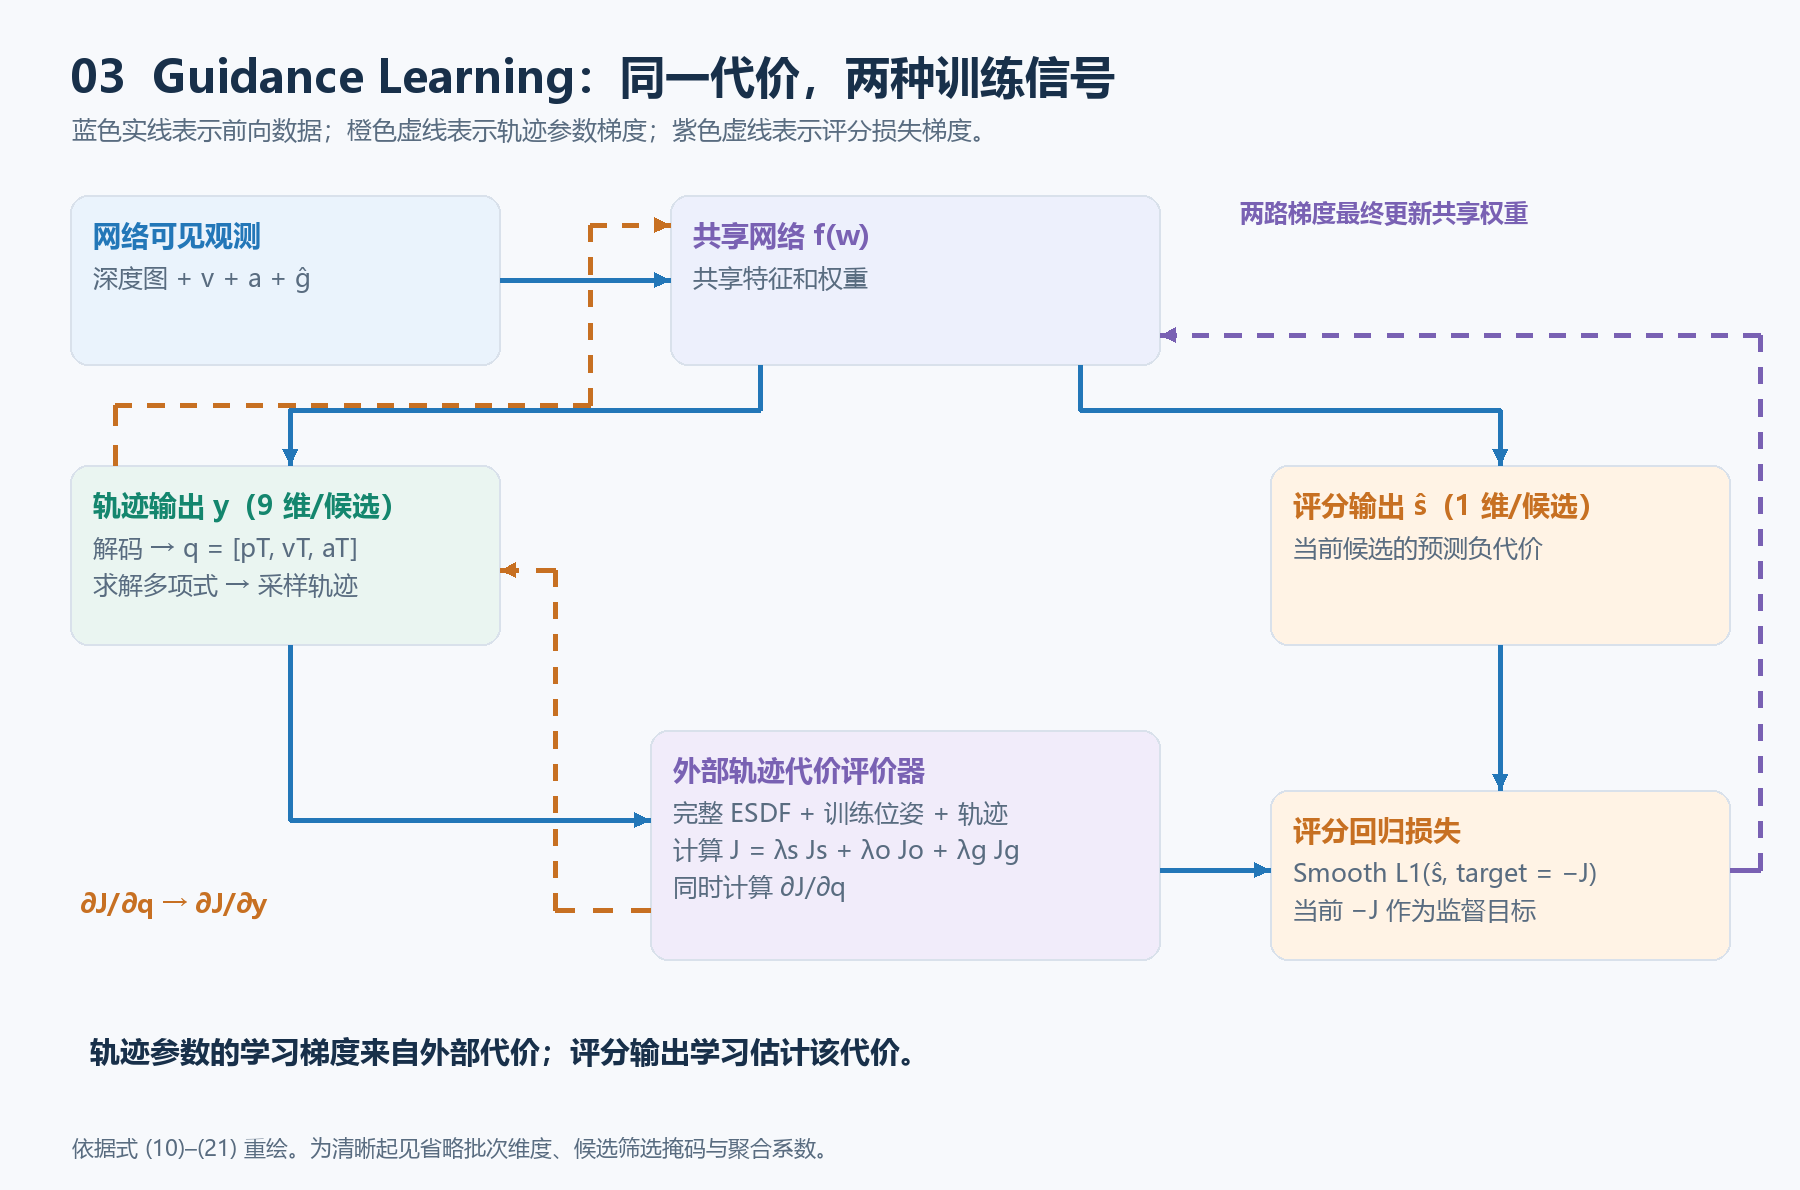
\includegraphics[width=\linewidth]{figures/22_note_training_gradients.png}
      \begin{center}\scriptsize\color{yopogray}
      笔记图 3：蓝色为前向数据流，橙色为轨迹参数梯度，
      紫色为评分损失梯度
      \end{center}
    \end{column}
    \begin{column}{0.4\textwidth}
      \small
      \begin{block}{路径一：轨迹参数}
        \footnotesize
        外部代价梯度 $\partial J/\partial\mathbf q$
        $\to$ 解码链 $\partial\mathbf q/\partial\mathbf y$
        $\to$ 共享网络权重。
        \textbf{这条路径不经过预测评分}——
        轨迹不是靠“评分告诉它该往哪改”来改进的。
      \end{block}
      \begin{block}{路径二：评分}
        \footnotesize
        预测评分与“当前候选的负代价”之间的回归误差，
        直接反向传播到评分通道（也会经共享骨干影响特征）。
      \end{block}
      \begin{reading}
        \scriptsize
        两条路径最终作用于\textbf{同一组权重}，
        因此是共同优化，而不是两个互不影响的网络。
      \end{reading}
    \end{column}
  \end{columns}
\end{frame}

% ---------------------------------------------------------------
\begin{frame}{评分输出的学习目标}
  \small
  \begin{columns}[t]
    \begin{column}{0.5\textwidth}
      原文式 (21)：轨迹评分定义为 $-J$，用 smooth $L_1$ 监督
      \[
        \mathcal L=\text{Smooth}L_1\bigl(y_s,\,-J\bigr)
      \]
      \begin{itemize}\tight
        \item $y_s$：网络预测的评分（共享特征上的第 10 个输出）；
        \item $-J$：由评价器\textbf{当场算出}的目标；
        \item 两者误差经普通反向传播回到评分通道。
      \end{itemize}
      \begin{paperfinding}[在线如何使用]
        \footnotesize
        部署时没有地图，无法计算 $J$，
        于是用预测评分代替真实的代价排序——
        选评分最高的候选（等价于代价最低）。
      \end{paperfinding}
    \end{column}
    \begin{column}{0.46\textwidth}
      \begin{reading}[“评分是不是一个独立回归问题”]
        \small
        形式上是一个回归，但\textbf{不独立}，有三重耦合：
        \begin{itemize}\tight
          \item \textbf{目标不是固定标签}：目标由网络自己当前的输出算出，
                网络一变、标签就变；
          \item \textbf{梯度进同一个骨干}：评分误差会改变共享特征，
                从而改变下一轮的轨迹输出；
          \item \textbf{它是评分通道唯一的监督}：没有它，第 10 个输出学不会。
        \end{itemize}
        真正被切断的只有一条：评分误差\textbf{不能直接把终端状态改掉}。
      \end{reading}
    \end{column}
  \end{columns}
\end{frame}

% ---------------------------------------------------------------
\begin{frame}{评分学习：数值算例}
  \footnotesize
  \begin{columns}[c]
    \begin{column}{0.56\textwidth}
      \begin{teach}[构造的两条候选（三个权重都取 1）]
        \scriptsize
        \begin{tabular}{@{}lrr@{}}
          \toprule
          项目 & 候选 A & 候选 B \\
          \midrule
          平滑 $J_s$ & 0.10 & 0.20 \\
          避障 $J_o$ & 0.70 & 0.05 \\
          目标 $J_g$ & 0.20 & 0.15 \\
          \midrule
          合计 $J$ & 1.00 & \textbf{0.40} \\
          目标 $-J$ & $-1.00$ & $-0.40$ \\
          当前预测 $\hat s$ & $-0.20$ & $-0.90$ \\
          \bottomrule
        \end{tabular}
      \end{teach}
      \begin{reading}
        \scriptsize
        当前预测会选 A，但按评价器应选 \textbf{B}——
        这正是评分误差要修正的排序错误。
        （论文实测：专家平均代价 0.078、网络训练后 0.050，
        候选间的代价差距远小于本表的教学数字。）
      \end{reading}
    \end{column}
    \begin{column}{0.4\textwidth}
      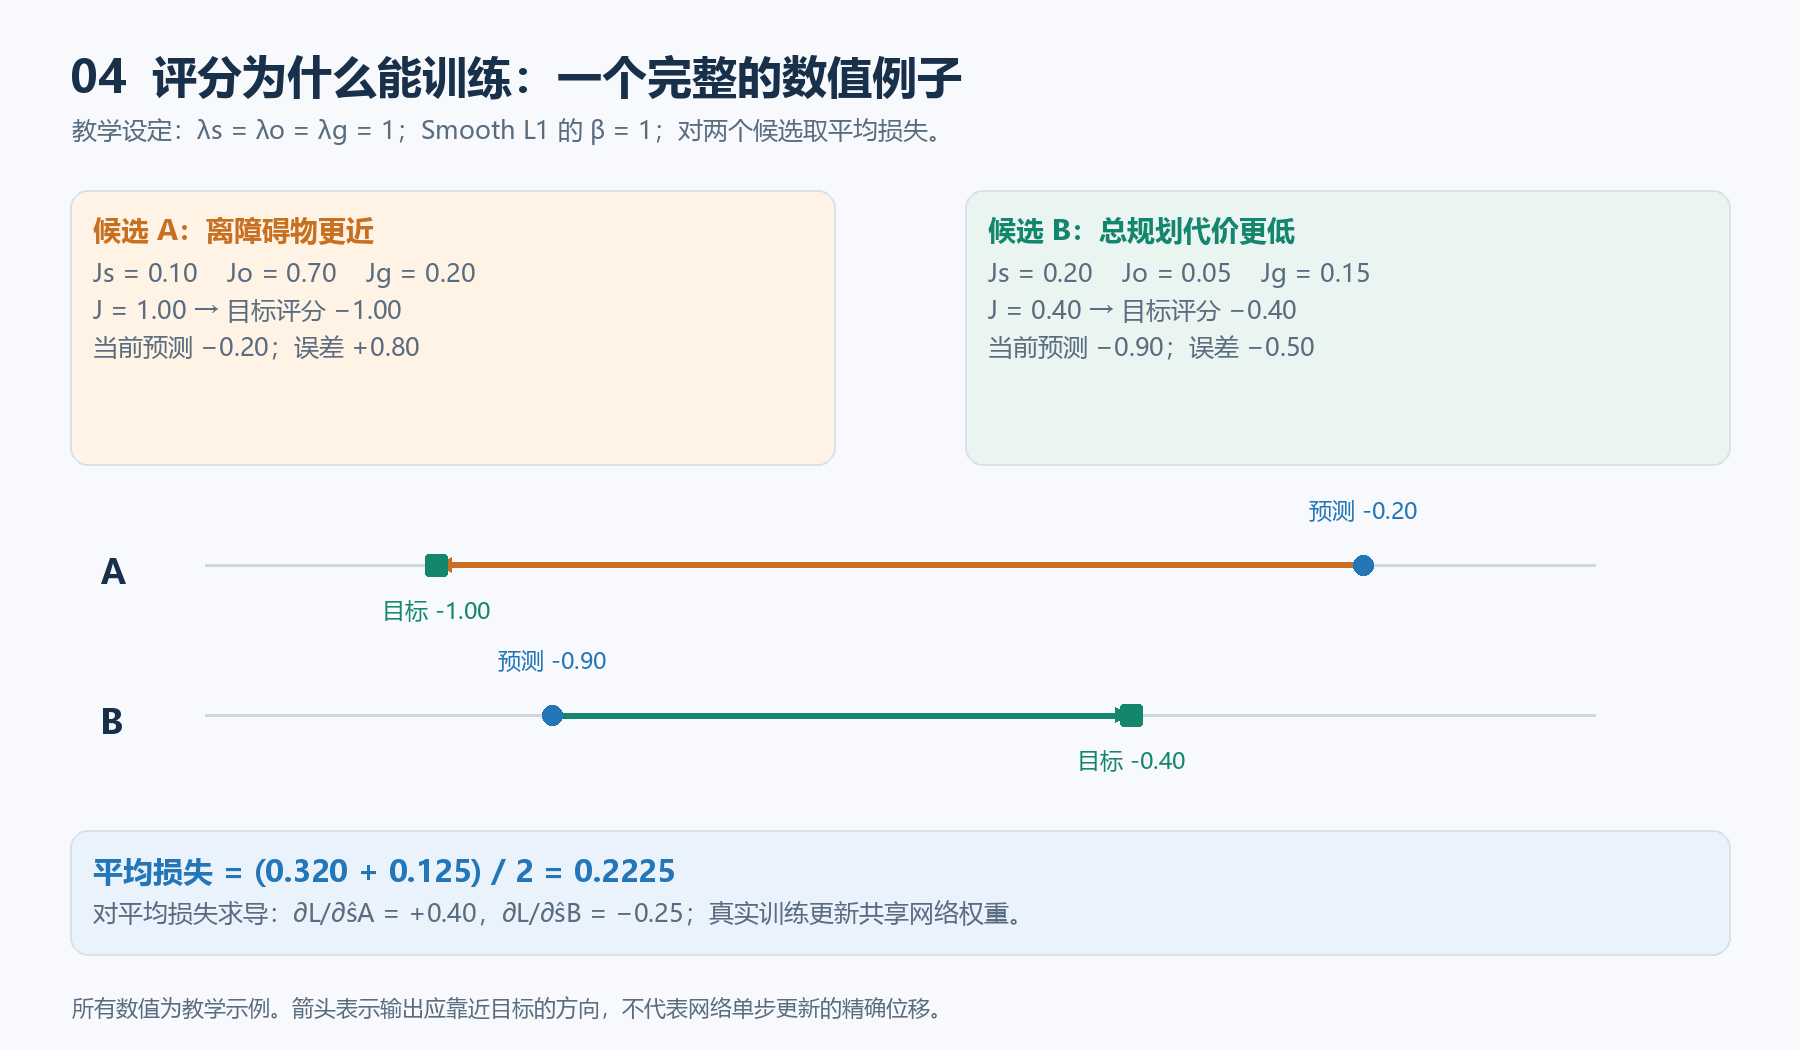
\includegraphics[width=\linewidth]{figures/23_note_score_learning.png}
      \begin{center}\scriptsize\color{yopogray}
      笔记图 4：蓝点为预测，绿方块为目标，
      箭头表示误差应减小的方向
      \end{center}
    \end{column}
  \end{columns}
\end{frame}

% ---------------------------------------------------------------
\begin{frame}{候选筛选策略}
  \small
  \begin{columns}[t]
    \begin{column}{0.5\textwidth}
      \begin{paperfinding}[原文的描述]
        \footnotesize
        \begin{itemize}\tight
          \item \textbf{所有}基元的预测评分都参与训练；
          \item 但只有\textbf{评分高于阈值}的候选，其终端状态才接受轨迹优化的训练；
          \item 实验阈值为 \textbf{0.04}；
          \item 阈值过小 $\to$ 过拟合到安全条件、整体不稳定；
                阈值过大 $\to$ 受负样本影响、难以收敛。
        \end{itemize}
      \end{paperfinding}
    \end{column}
    \begin{column}{0.46\textwidth}
      \begin{reading}[候选筛选的作用]
        \small
        代价很高的候选（例如直接朝向障碍）其梯度方向参考价值有限，
        让它参与“把终点往哪推”的学习可能引入噪声。
        因此：\textbf{评分继续学全部候选，轨迹参数只学可救的那部分}。
      \end{reading}
      \begin{reading}[记号方向的注意事项]
        \scriptsize
        原文把评分定义为 $-J$（越大越好），
        所以“评分高于阈值”与“代价低于阈值”是同一件事。
        阅读时需注意符号方向，避免误读为“训练代价最大的候选”。
      \end{reading}
    \end{column}
  \end{columns}
\end{frame}

% ---------------------------------------------------------------
\begin{frame}[shrink=6]{特权学习：训练与部署的信息差异}
  \begin{columns}[c]
    \begin{column}{0.62\textwidth}
      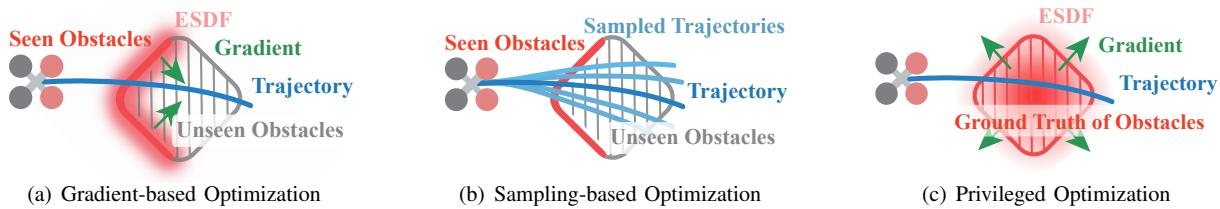
\includegraphics[width=0.94\linewidth]{figures/06_privileged_learning.jpg}
      \begin{center}\scriptsize\color{yopogray}
      原文 Fig.~6：(a) 梯度法、(b) 采样法、
      (c) 特权优化——前两者会被遮挡或初始值困住
      \end{center}
    \end{column}
    \begin{column}{0.36\textwidth}
      \small
      \begin{block}{训练时可访问}
        \footnotesize
        \begin{itemize}\tight
          \item 完整点云与 ESDF 地图；
          \item 无人机完整状态（位置、姿态）；
          \item 用于计算代价与梯度。
        \end{itemize}
      \end{block}
      \begin{block}{部署时只有}
        \footnotesize
        \begin{itemize}\tight
          \item 噪声深度图；
          \item 速度、加速度、目标方向；
          \item 状态估计给出的当前位置。
        \end{itemize}
      \end{block}
      \begin{reading}
        \scriptsize
        特权信息\textbf{不进入网络输入}，
        只用于产生监督。因此部署仍受有限视野与部分可观测性限制，
        但其学习信号来自完整环境。
      \end{reading}
    \end{column}
  \end{columns}
\end{frame}

% ---------------------------------------------------------------
\begin{frame}{数据与训练配置}
  \small
  \begin{columns}[t]
    \begin{column}{0.5\textwidth}
      \begin{block}{原文给出的训练设置}
        \footnotesize
        \begin{tabular}{@{}ll@{}}
          \toprule
          数据集 & Flightmare 中随机重置状态采集 \\
          样本量 & 约 \textbf{100K} \\
          迭代 & \textbf{50} 个 epoch \\
          批量大小 & \textbf{16} \\
          学习率 & $1.5\times10^{-4}$ \\
          优化器 & Adam \\
          无效深度 & 最近邻插值填充 \\
          进一步微调 & 数据聚合（DAgger）\\
          \bottomrule
        \end{tabular}
      \end{block}
    \end{column}
    \begin{column}{0.46\textwidth}
      \begin{paperfinding}[无需重新标注的原因]
        \small
        同一张深度图可以配\textbf{不同的速度、加速度与目标方向}，
        每次都重新计算代价即可——
        不需要重新生成专家轨迹标签，也不需要重新与仿真器交互。
        这是“无专家”带来的数据增广能力。
      \end{paperfinding}
      \begin{reading}[“无监督”的准确含义]
        \scriptsize
        不依赖\textbf{专家最优轨迹示范}，
        但依赖\textbf{人为设计的代价、环境特权信息}与\textbf{计算出的监督信号}。
        与“没有任何监督信号”不是一回事。
      \end{reading}
    \end{column}
  \end{columns}
\end{frame}

% ---------------------------------------------------------------
\begin{frame}{训练与推理的数据流对照}
  \scriptsize
  \begin{center}
  \begin{tabular}{@{}p{0.22\textwidth}p{0.335\textwidth}p{0.335\textwidth}@{}}
    \toprule
    \textbf{环节} & \textbf{训练阶段} & \textbf{在线推理阶段} \\
    \midrule
    网络输入 & 深度、速度、加速度、目标方向 & 相同类型的可观测输入 \\
    \addlinespace
    网络输出 & 15 组参数与评分 & 15 组参数与评分 \\
    \addlinespace
    候选轨迹求解 & 为计算代价与梯度，\textbf{15 条都要生成} & 只需求解\textbf{被选中的那一条} \\
    \addlinespace
    完整地图与位姿 & 供外部评价器计算代价与梯度 & 在线规划\textbf{不依赖}训练用完整 ESDF \\
    \addlinespace
    规划代价 $J$ & 直接计算并指导训练 & 用\textbf{预测评分}估计质量 \\
    \addlinespace
    反向传播 & 两种信号更新共享权重 & 无 \\
    \addlinespace
    控制器执行 & 主训练反馈\textbf{不要求}逐条闭环执行 & 跟踪选中轨迹、持续重规划 \\
    \bottomrule
  \end{tabular}
  \end{center}
  \vspace{0.2em}
  \begin{reading}
    \scriptsize
    需注意“候选轨迹求解”一行：
    训练时 15 条均需解出多项式方可计算代价，在线时仅求解 1 条。
  \end{reading}
\end{frame}

% ============================ 03 实验 ============================

\section{实验验证}

\begin{frame}[plain]
  \begin{center}
    \vspace{1.2cm}
    {\color{yopoblue}\Huge\bfseries 03}\\[0.5em]
    {\color{yopoblue}\LARGE 实验验证}\\[1.2em]
    \begin{minipage}{0.76\textwidth}
      \small\color{yopogray}
      本部分仅陈述原文可支持的结论及其边界。
      平台、密度、速度等前提均予保留，不同条件下的数字不直接比较。
    \end{minipage}
  \end{center}
\end{frame}

% ---------------------------------------------------------------
\begin{frame}{与梯度优化专家的对比}
  \small
  \begin{columns}[t]
    \begin{column}{0.56\textwidth}
      \begin{block}{原文表 I（PDF 第 6 页）}
        \footnotesize
        \begin{tabular}{@{}llrr@{}}
          \toprule
          方法 & 指标 & 代价 & 耗时 \\
          \midrule
          专家（50 步梯度下降） & 平均 & 0.078 & \multirow{2}{*}{30\,ms} \\
                                & 最优 & 0.036 & \\
          \addlinespace
          网络（初始） & 平均 & 0.105 & \multirow{4}{*}{1.6\,ms} \\
          网络（初始） & 最优 & 0.056 & \\
          网络（训练后） & 平均 & \textbf{0.050} & \\
          网络（训练后） & 最优 & \textbf{0.036} & \\
          \bottomrule
        \end{tabular}
      \end{block}
      \begin{reading}[“专家”的含义]
        \scriptsize
        指同一代价函数下的\textbf{经典梯度下降优化器}，
        从基元初值出发迭代 50 步。
        它是模仿学习里“提供示范”的那个上界，而不是 YOPO 训练的一部分。
      \end{reading}
    \end{column}
    \begin{column}{0.42\textwidth}
      \begin{reading}[结论适用范围]
        \small
        \begin{itemize}\tight
          \item 网络学到了有效的\textbf{快速映射}：
                耗时降低一个数量级以上；
          \item 在\textbf{平均候选代价}上优于所比较的专家；
          \item 最优候选代价与专家接近。
        \end{itemize}
      \end{reading}
      \begin{reading}[结论的边界]
        \small
        \begin{itemize}\tight
          \item 不能证明优于所有优化器；
          \item 不构成全局最优保证；
          \item 不能外推到未测试的初始条件分布。
        \end{itemize}
      \end{reading}
    \end{column}
  \end{columns}
\end{frame}

% ---------------------------------------------------------------
\begin{frame}{与 SOTA 方法对比：延迟、安全性与平滑性}
  \small
  \begin{center}\scriptsize
  \begin{tabular}{@{}lccccccc@{}}
    \toprule
    \multirow{2}{*}{方法} & 密度 & \multicolumn{4}{c}{延迟 / ms} &
    \multicolumn{2}{c}{障碍距离 / m} \\
    \cmidrule(lr){3-6}\cmidrule(lr){7-8}
     & (tree/m$^2$) & 建图 & 前端 & 后端 & \textbf{总计} & 平均 & 最小 \\
    \midrule
    \multirow{2}{*}{TopoTraj} & 1/30 & \multirow{2}{*}{48.5} & \multirow{2}{*}{6.1} & \multirow{2}{*}{7.3} & \multirow{2}{*}{61.9} & 1.23 & 0.18 \\
                              & 1/20 & & & & & 1.00 & 0.08 \\
    \addlinespace
    \multirow{2}{*}{MPPI} & 1/30 & \multirow{2}{*}{6.5} & \multirow{2}{*}{5.0} & \multirow{2}{*}{8.2} & \multirow{2}{*}{19.7} & 1.23 & 0.08 \\
                          & 1/20 & & & & & 0.94 & 0.06 \\
    \addlinespace
    \multirow{2}{*}{Agile Autonomy} & 1/30 & \multirow{2}{*}{/} & \multirow{2}{*}{/} & \multirow{2}{*}{/} & \multirow{2}{*}{5.4} & 1.13 & 0.12 \\
                                   & 1/20 & & & & & 1.01 & 0.10 \\
    \addlinespace
    \multirow{2}{*}{\textbf{YOPO}} & 1/30 & \multirow{2}{*}{/} & \multirow{2}{*}{/} & \multirow{2}{*}{/} & \multirow{2}{*}{\textbf{1.6}} & \textbf{1.63} & \textbf{0.24} \\
                                   & 1/20 & & & & & \textbf{1.28} & \textbf{0.16} \\
    \bottomrule
  \end{tabular}
  \end{center}
  \vspace{0.1em}
  \begin{reading}
    \footnotesize
    平台为 i7-9700 + RTX 3060，平均速度 4\,m/s。
    此设置下 YOPO 的\textbf{障碍间距最好}；
    但 MPPI 的\textbf{平滑性}更好（其平滑性代价 16.83\,m$^2$/s$^5$ 远低于 YOPO 的 73.52）。
    高速度、密集场景下 Agile Autonomy 更有竞争力——
    不能写成“YOPO 在所有速度和指标上都最优”。
  \end{reading}
\end{frame}

% ---------------------------------------------------------------
\begin{frame}{速度-成功率曲线与轨迹对比}
  \small
  \begin{columns}[c]
    \begin{column}{0.58\textwidth}
      \begin{tabular}{@{}cc@{}}
        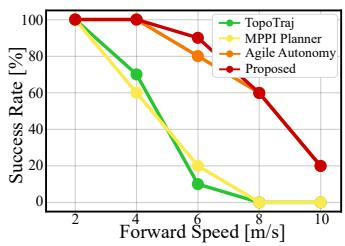
\includegraphics[width=0.47\linewidth]{figures/07a_success_sparse.jpg} &
        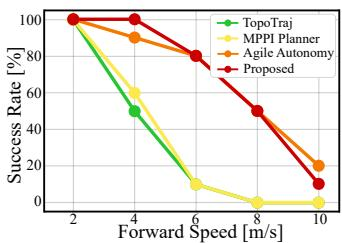
\includegraphics[width=0.47\linewidth]{figures/07b_success_dense.jpg}\\
        \scriptsize (a) 稀疏：1/30 tree/m$^2$ &
        \scriptsize (b) 密集：1/20 tree/m$^2$ \\
      \end{tabular}
      \begin{center}\scriptsize\color{yopogray}
      原文 Fig.~7：前飞速度 2--10\,m/s 的成功率，每个条件重复 10 次
      \end{center}
    \end{column}
    \begin{column}{0.4\textwidth}
      \footnotesize
      \begin{itemize}\tight
        \item 两种密度下，学习式方法的成功率\textbf{显著高于}经典视觉方法；
        \item 经典基线下降的原因：传感器量程有限、深度噪声、
              地图不完整；而概率式地图更新虽然能去噪，却让重建变慢；
        \item YOPO 在 \textbf{6\,m/s 以下}优于 Agile Autonomy，
              因为它并行预测更多拓扑不同的候选；
        \item 由于训练时考虑了平滑性，高速密集场景下会牺牲一部分安全性。
      \end{itemize}
    \end{column}
  \end{columns}
  \vspace{0.2em}
  \begin{center}
  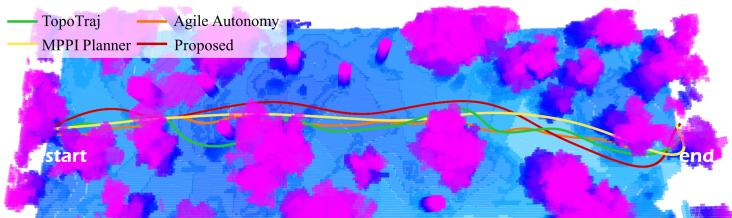
\includegraphics[width=0.46\linewidth]{figures/08a_trajectory_sparse.jpg}\hfill
  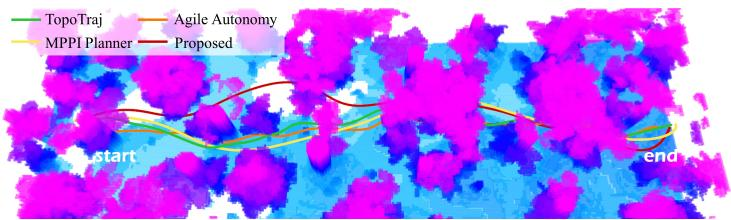
\includegraphics[width=0.46\linewidth]{figures/08b_trajectory_dense.jpg}
  \end{center}
  \begin{center}\scriptsize\color{yopogray}
  原文 Fig.~8：稀疏与密集森林中的轨迹对比
  \end{center}
\end{frame}

% ---------------------------------------------------------------
\begin{frame}{真机平台与机载配置}
  \small
  \begin{columns}[c]
    \begin{column}{0.5\textwidth}
      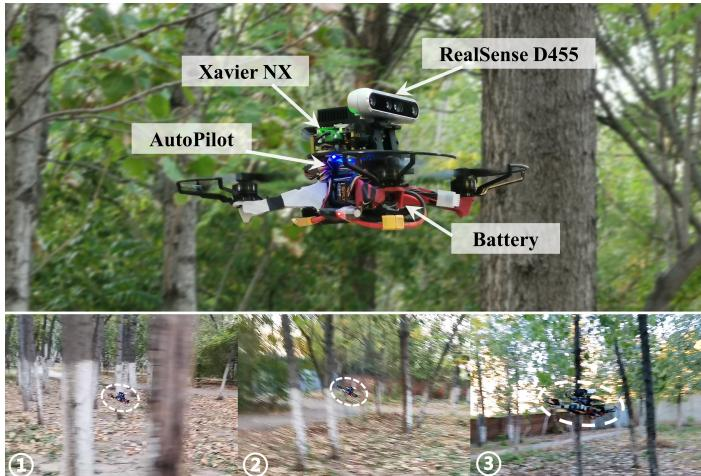
\includegraphics[width=\linewidth]{figures/09_platform.jpg}
      \begin{center}\scriptsize\color{yopogray}
      原文 Fig.~9：物理平台与真机实验场景
      \end{center}
    \end{column}
    \begin{column}{0.46\textwidth}
      \begin{block}{机载配置}
        \scriptsize
        \begin{itemize}\tight
          \item 250\,mm 轴距、1.13\,kg 四旋翼；
          \item RealSense D455 深度相机
                （$87^\circ\times58^\circ$，约 6\,m 量程）；
          \item VINS-Fusion 状态估计；
          \item Xavier NX 机载计算，TensorRT 部署后约 \textbf{16\,ms}；
          \item 几何控制器跟踪参考轨迹。
        \end{itemize}
      \end{block}
      \begin{reading}[相机与网络的衔接]
        \scriptsize
        真机图像宽高比 16:9，被缩放到 $160\times96$ 后输入网络；
        无效深度用最近邻插值填充，与训练时的处理保持一致。
      \end{reading}
    \end{column}
  \end{columns}
\end{frame}

% ---------------------------------------------------------------
\begin{frame}{真机飞行结果}
  \small
  \begin{center}
    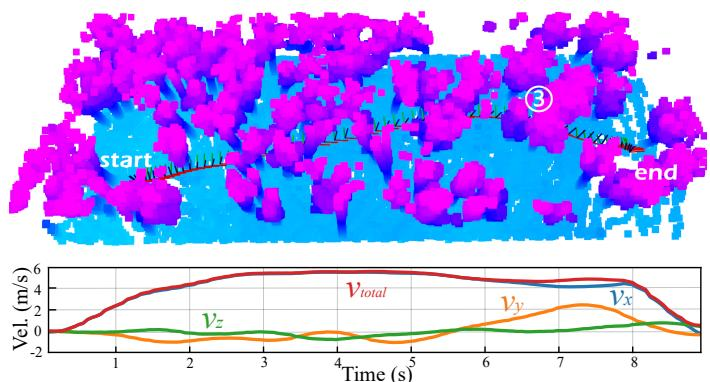
\includegraphics[width=0.66\linewidth]{figures/10c_map_and_velocity.jpg}
  \end{center}
  \vspace{-0.4em}
  \begin{center}\scriptsize\color{yopogray}
  原文 Fig.~10：真机飞行轨迹与速度曲线（地图仅用于展示，飞行中并不使用）
  \end{center}
  \vspace{0.2em}
  \begin{columns}[t]
    \begin{column}{0.48\textwidth}
      \begin{reading}[两个延迟指标的区分]
        \scriptsize
        桌面端 1.6\,ms 与机载 16\,ms 属于\textbf{不同平台}；
        二者都不能直接当作整条感知—规划—控制链路的端到端延迟。
      \end{reading}
    \end{column}
    \begin{column}{0.48\textwidth}
      \begin{reading}[飞行条件]
        \scriptsize
        最高速度 \textbf{5.52\,m/s}；实验森林密度 1/10 tree/m$^2$、
        树径约 0.25\,m；该环境在训练时\textbf{从未被观测过}。
      \end{reading}
    \end{column}
  \end{columns}
\end{frame}

% ============================ 04 小结 ============================

\section{小结、易错点与待核对项}

\begin{frame}{主要结论}
  \scriptsize
  \begin{block}{一、前向推理：网络预测的是“修正量”，不是轨迹}
    \scriptsize
    候选 $=$ 固定锚点 $+$ \textbf{网络预测的有界偏移与终端导数}；
    曲线由“当前状态 $+$ 终端状态”代入五次多项式边界值问题\textbf{解析求出}。
    在线只解被选中的一条；输入以\textbf{深度图为主}，状态次之，
    且状态会被旋转到 15 个基元系各一份。
  \end{block}
  \begin{block}{二、引导训练：监督来自“可求导的代价”，不是专家}
    \scriptsize
    评价器是手写的代价函数 $+$ 特权地图查询：
    平滑项与目标项给\textbf{闭式}梯度，避障项给\textbf{数值}梯度。
    自定义 autograd 层把 $\partial J/\partial\mathbf q$ 接进计算图，
    链式法则沿“解码链 $\to$ 网络权重”完成更新。
  \end{block}
  \begin{block}{三、两种输出、两条信号，一套权重}
    \scriptsize
    轨迹参数靠\textbf{外部代价梯度}改进（不经过预测评分）；
    评分靠\textbf{回归当前代价}学会排序；
    两者作用于共享骨干，是联合优化而非两个独立网络。
  \end{block}
\end{frame}

% ---------------------------------------------------------------
\begin{frame}{易混淆概念对照}
  \scriptsize
  \begin{center}
  \begin{tabular}{@{}p{0.33\textwidth}p{0.6\textwidth}@{}}
    \toprule
    \textbf{常见但不准确的理解} & \textbf{准确理解} \\
    \midrule
    15 个固定动作中选一个 & 固定的是锚点，终点是可预测的 \\
    15 个区域各运行搜索线程 & 共享网络并行产生多个空间位置的输出 \\
    只输出 2\,s 后的位置 & 还输出终端速度、加速度与评分 \\
    网络直接输出多项式系数 & 输出边界参数，系数由解析映射得到 \\
    在线生成全部曲线再查地图评分 & 参数与评分同时预测，只求解选中曲线 \\
    轨迹分支经“学出的评分”反传 & 主轨迹梯度来自外部代价评价器 \\
    无监督 $=$ 没有监督信号 & 无专家轨迹标签，但有代价与评分目标 \\
    终端限幅 $\Rightarrow$ 全程安全可执行 & 限幅与软代价改善表现，非全程硬约束证明 \\
    特权训练让网络知晓所有遮挡 & 部署仍受有限视野与部分可观测性限制 \\
    \bottomrule
  \end{tabular}
  \end{center}
  \vspace{0.2em}
  \begin{reading}
    \scriptsize
    由此可进一步推论：遇到严重遮挡、异常观测或训练分布之外的场景时，
    快速预测的评分可能失准。原文证明了特定场景中的有效性，
    \textbf{没有给出任意未知环境的完整安全保证}。
  \end{reading}
\end{frame}

% ---------------------------------------------------------------
\begin{frame}{待核对事项}
  \small
  \begin{columns}[t]
    \begin{column}{0.5\textwidth}
      \begin{block}{实现层面待确认}
        \footnotesize
        \begin{itemize}\tight
          \item 代价权重、归一化与时间采样间隔；
          \item 终端导数缩放的分量含义与坐标变换约定；
          \item 评分目标的符号、筛选阈值与比较方向；
          \item 自定义梯度、评分目标的停止梯度、聚合尺度；
          \item 重规划起点来自当前估计还是旧参考，
                以及拼接处的连续性。
        \end{itemize}
      \end{block}
    \end{column}
    \begin{column}{0.46\textwidth}
      \begin{block}{验证层面待确认}
        \footnotesize
        \begin{itemize}\tight
          \item 用简单障碍场景比较有限差分与解析/数值梯度；
          \item 轨迹表示换成其他参数化（如 MINCO）后，
                梯度的哪一段会失效；
          \item 论文与公开代码在评分符号、候选筛选、时域上的差异需要逐一记录。
        \end{itemize}
      \end{block}
      \begin{reading}
        \scriptsize
        作者仓库已有后续重构版本与不同轨迹表示的分支，
        参考时\textbf{应记录具体 commit}，
        避免把新版表示或部署指标写回 2024 年原文。
      \end{reading}
    \end{column}
  \end{columns}
\end{frame}

% ---------------------------------------------------------------
\begin{frame}{来源与说明}
  \small
  \begin{columns}[t]
    \begin{column}{0.5\textwidth}
      \begin{block}{本报告的依据}
        \footnotesize
        \begin{itemize}\tight
          \item 原文 PDF：\texttt{YOPO\_original.pdf}（8 页）；
                页码指该 PDF 页序，非期刊页码；
          \item 阅读笔记：\texttt{YOPO/papernote.md}（2026-10-08 版）；
          \item 原文配图：MinerU 提取结果中的图像文件；
          \item 笔记配图：由笔记作者绘制的教学示意图。
        \end{itemize}
      \end{block}
    \end{column}
    \begin{column}{0.46\textwidth}
      \begin{reading}[三类内容的标注]
        \footnotesize
        \begin{itemize}\tight
          \item \textbf{蓝色块}：原文可查证的结论，已注明图/表/式编号；
          \item \textbf{绿色块}：为便于理解构造的教学数字，
                不是论文实验数据；
          \item \textbf{橙色块}：本笔记的整理与推论，
                与原文陈述需区分。
        \end{itemize}
      \end{reading}
    \end{column}
  \end{columns}

  \vspace{0.4em}
  \begin{center}
    \Large\color{yopoblue}\bfseries 谢谢，欢迎讨论
  \end{center}
\end{frame}


\end{document}
